
\documentclass[conference,compsoc]{IEEEtran}
\usepackage{graphicx}
\usepackage{amsfonts}
\usepackage{amsmath}

\graphicspath{ {./images/} }



\begin{document}

\title{Physics Informed Neural Networks (PINNs): Review}

\author{\IEEEauthorblockN{Atharva Mahesh Kavitkar}
\IEEEauthorblockA{Department of Computer Science}
\IEEEauthorblockA{Technische Universit\"{a}t Kaiserslautern}
\IEEEauthorblockA{kavitkar@rhrk.uni-kl.de}}

\maketitle


\begin{abstract}
Despite significant advances in numerically modeling multiphysics systems, it is still not possible to effectively incorporate noisy data into current techniques. Furthermore, addressing inverse problems with hidden physics is sometimes prohibitively costly, demanding several formulations and complex computer algorithms. Machine learning has emerged as a viable alternative, however deep neural network training needs large amounts of data, which is not always accessible for scientific issues. Rather, such networks may be developed using new data collected by imposing physical laws. This type of physics-informed learning incorporates (noisy) data with mathematical models, which are then implemented using neural networks or other kernel-based regression networks. Furthermore, customized network architectures that automatically meet certain of the physical invariants for higher accuracy, faster training, and enhanced generalization may be plausible. This review discusses some of the current trends in integrating physics into deep learning, as well as some of the current deep learning architectures, how they work, and the results obtained on various applications of physics- informed learning, both forward and inverse, such as discovering hidden physics and tackling high-dimensional problems.

\end{abstract}

\section{Introduction}
% no \IEEEPARstart


Machine learning algorithms have become the standard methodology for all types of data analytics due to the availability of data\cite{raissi2019physics}\cite{lou2020physics}\cite{karniadakis2021physics}. However, the expense of data gathering is considerable when working with complicated physical systems \cite{cai2021physics}. As a result, the machine learning algorithms that have been built must make decisions based on incomplete information\cite{karniadakis2021physics}. Such machine learning approaches (for example, deep/recurrent/convolution neural networks) lack resilience and cannot guarantee convergence\cite{raissi2019physics}.


\begin{figure}[h]
    \centering
    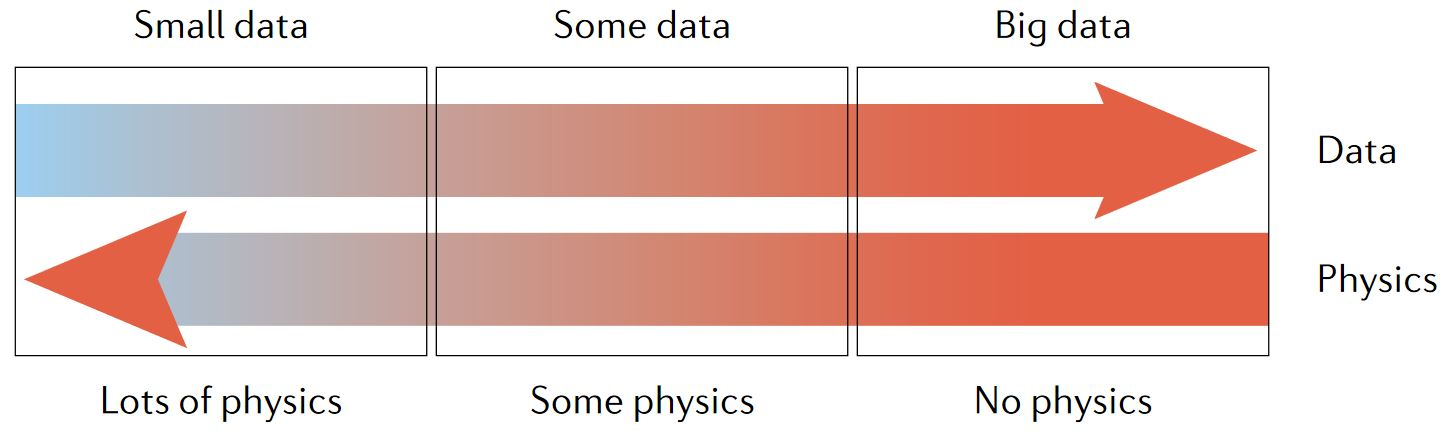
\includegraphics[scale=0.5,width = 8cm]{figures/data_vs_physics.JPG}
    \caption{Categories of physics problems vs. available data\cite{karniadakis2021physics}}
\end{figure}

The chart above illustrates three distinct sorts of physical problems, as well as the associated data\cite{karniadakis2021physics}.
All of the physics is assumed to be known in the small data regime, and data for the initial and boundary conditions, as well as the coefficients of a partial differential equation, are given.
The intermediate regime is most prevalent in applications where one knows certain data and fundamental physics but is missing certain parameter values or even a full term in the partial differential equation\cite{raissi2019physics}. Finally, there is the big data regime, where one may not understand any of the physics and where a data-driven technique, such as using operator regression methods to reveal unknown physics, may be most effective\cite{karniadakis2021physics}. Using physics-informed machine learning, data and the underlying physical principles, even models with partially missing physics, may be seamlessly incorporated\cite{cai2021physics}\cite{karniadakis2021physics}. Automatic differentiation and neural networks, which are designed to offer predictions that adhere to the underlying physical principles, can be used to express this in a succinct manner\cite{raissi2019physics}. 

Vanilla physics informed neural networks have been deployed in various biological and physical domains such as material science and fluid dynamics \cite{cai2021physics}\cite{tipireddy2019comparative}\cite{erichson2019physics}\cite{reyes2021learning}\cite{tartakovsky2020physics}. Apart from that, the advancements in the PINNs architecture can be classified in two broad approaches. One approach is to optimise the current Vanilla PINN architecture by incorporating techniques such as attention mechanism, gradient pathology\cite{wang2020understanding}\cite{hospedales2020meta}, dynamic activation functions etc\cite{jagtap2020locally}\cite{jagtap2020adaptive}\cite{elsken2019neural}. The other approach has been to come up with completely new architectures based on the Vanilla PINN architecture. A few such architectures are f-pinns\cite{pang2019fpinns}, c-PINNs, PhyGeoNet\cite{gao2021phygeonet}, V-PINNs, hp-VPINNs etc\cite{shukla2021parallel}.

The idea of using a deep neural network on few potentially high dimensional datapoints to approximate a non linear mapping seems impractical\cite{karniadakis2021physics}. For the moment, advanced machine learning algorithms for modeling physical and biological systems aren't taking into account the vast quantity of past knowledge that's available to them\cite{cai2021physics}. The effective information from the same amount of data is increased when such structured knowledge is also utilised in the training process\cite{karniadakis2021physics}.This aids the network to converge faster to the optimal solution and also generalise well given the limited amount of data\cite{karniadakis2021physics}\cite{mishra2020estimates}.

%%%%%%%%%%%%%%%%%%%%%%%%%
The remainder of this paper is organized as follows. The background section explains the working of Vanilla PINNs in detail. The advantages of having a physics informed part along with the limitations of Vanilla PINNs architecture are discussed. Advanced PINN approaches discuss the more complex PINN architectures being used to overcome limitations of Vanilla PINNs. Conclusion andfuture work are outlined in the last section of the paper.
%%%%%%%%%%%%%%%%%%%%%%%%

\section{Background}
In this section, we'll go through the basics of the PINN idea before moving on to more recent developments.
\begin{figure*}[h]
    \centering
    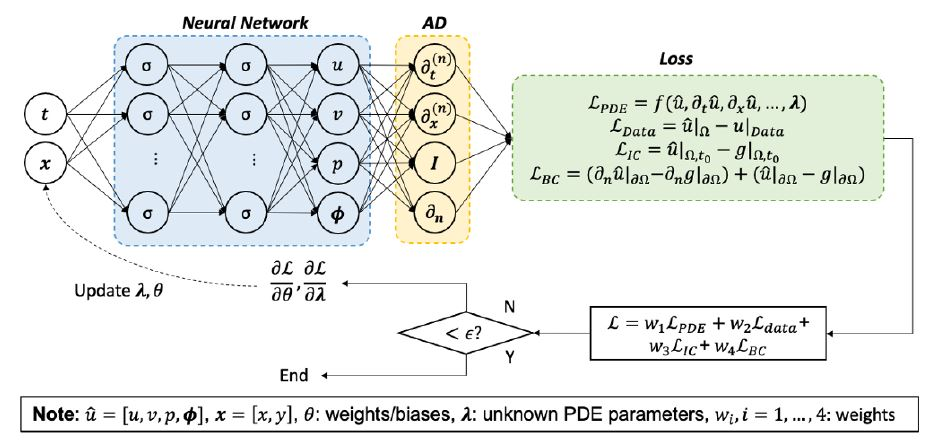
\includegraphics[scale=0.8]{figures/PINN_architecture.JPG}
    \caption{Vanilla PINN architecture\cite{raissi2019physics}}
\end{figure*}

Consider a parametrized partial differential equation (PDE) system with the following equations:

\begin{equation}
   f(x,t,\hat{u},\partial_x\hat{u},\partial_t\hat{u},...,\lambda) = 0, x\in\Omega, t \in [0,T] 
\end{equation}

\begin{equation}
    \hat{u}(x,t_0) = g_0(x) x\in\Omega ,
\end{equation}

\begin{equation}
    \hat{u}(x,t) = g_\Gamma(t) x\in \partial\Omega , t \in [0,T],
\end{equation}

where $x \in \mathbb{R}^d$ is the spatial coordinate and t is the time; $f$ denotes the residual of the PDE, containing the differential operators (i.e. $[\partial_x\hat{u},\partial_t\hat{u},...]); \mathbb{\lambda} = [\lambda_1,\lambda_2,...]$ are the PDE parameters; $\hat{u}(x,t)$ is the solution of the PDE with initial condition $g_0(x)$ and boundary equation $g_\Gamma(t)$ (which can be Dirichlet, Neumann or mixed boundary condition)\cite{raissi2019physics};
$\Omega$ and $\partial\Omega$ represent the spatial domain and the boundary,respectively.
In the context of the vanilla PINNs, a
fully-connected feed-forward neural network, which is
composed of multiple hidden layers, is used to approximate
the solution of the PDE $\hat{u}$ by taking the space and time
coordinates (x; t) as inputs, as shown in the blue panel in Fig.2\cite{raissi2019physics}. Let the hidden variable of the $k^{th}$ hidden layer be
denoted by $z^k$, then the neural network can be expressed as

\begin{equation}
    z^0 = (x,t),
\end{equation}

\begin{equation}
    z^k = \sigma(W^kz^{k-1} + b^k), 1 \leq k \leq L-1
\end{equation}

\begin{equation}
    z^k = W^kz^{k-1} + b^k, k=L,
\end{equation}

where the output of the last layer is used to approximate the
true solution, namely $\hat{u} \approx z^L$. $W^k$ and $b^k$ denote the weight matrix and bias vector of the $k^{th}$ layer; $\sigma(.)$ is a nonlinear
activation function. All the trainable model parameters, i.e.,
weights and biases, are denoted by $\theta$\cite{raissi2019physics}.

In PINNs, solving a PDE system (denoted by eq. 1) is
converted into an optimization problem by iteratively
updating $\theta$ with the goal to minimize the loss function L:

\begin{equation}
    L = \omega_1L_{PDE} + \omega_2L_{data} + \omega_3L_{IC} + \omega_4L_{BC},
\end{equation}

where $\omega_{1-4}$ are the weighting coefficients for different loss
terms. The first term $L_{PDE}$ in equ. 3 penalizes the residual
of the governing equations. The other terms are imposed to
satisfy the model predictions for the measurements $L_{data}$,
the initial condition $L_{IC}$, and the boundary condition $L_{BC}$,
respectively. In general, the mean square error (MSE),
taking the L2-norm of the sampling points, is employed to
compute the losses in equ. 3. A schematic of PINNs is shown in Fig. 2, where the key
elements (e.g., neural network, AD, loss function) are
indicated in different colors.



Since there are so many spatio-temporal degrees of freedom in modeling issues requiring long-time integration of PDEs, the quantity of data needed to train the PINN may be rather large as well\cite{raissi2019physics}. As a result, long-term physical difficulties will require the usage of PINNs, which may be computationally challenging \cite{cai2021physics}. PINNs have a high training cost, which might have a detrimental influence on their performance, especially when dealing with real-world situations that need a PINN model to function in real-time\cite{raissi2019physics}. The convergence of these models must thus be accelerated without losing performance.


\section{Advanced PINN approaches}

\subsection{Extended PINNs}
Finite-element techniques for solving governing physical laws in the form of partial differential equations on parallel computers have been transformed via domain decomposition\cite{jagtap2020extended}\cite{goswami2019transfer}. Most of these domains are separated by boundaries, and they only interact when they share a common boundary with other domains that meet certain continuity requirements. By solving a series of unrelated sub-problems, the global answer can be found.

For the eXtended PINNs (XPINNs), generalized domain decomposition is used\cite{jagtap2020extended}. To achieve high computational efficiency, this type of domain decomposition makes it easier to parallelize the network\cite{jagtap2020conservative}\cite{jagtap2020extended}. For example, XPINN offers all the features of cPINN, such as parallelization and a huge representation capacity. There are shallow neural networks for smooth zones and deep neural networks for areas where complicated solutions are expected\cite{jagtap2020extended}.

\begin{figure*}[h]
    \centering
    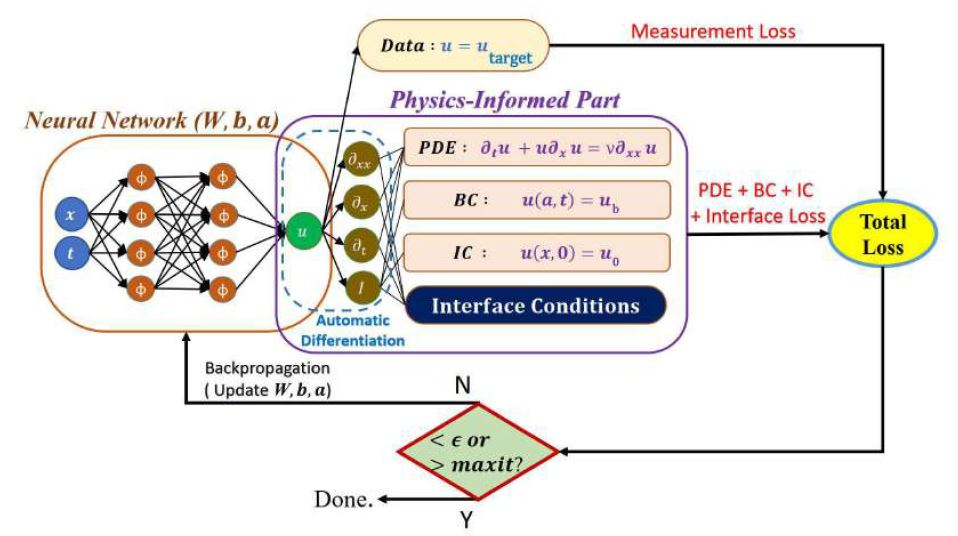
\includegraphics[scale = 0.8]{figures/xpinn.JPG}
    \caption{XPINN architecture\cite{jagtap2020extended}}
\end{figure*}

As shown in Fig. 3, additional interface conditions contribute to the loss function alongside DNN and PDE components in XPINN architecture. As part of XPINN's interface requirements, the residual continuity condition in strong form is enforced, as is the average solution provided by distinct Sub-Nets along the same interface.

\subsubsection{Working} 
Consider the computational domain, which is divided into $N_{sd}$ number of non overlapping
regular/irregular subdomains\cite{jagtap2020extended}. In the XPINN framework, the output of the
neural network in the $q^{th}$ subdomain is given by

\begin{equation}
    u_{\hat{\Theta}_q}(z) = \mathcal{N}(z;\hat{\Theta}_q) \in \Omega_q, q=1,2,...,N_{sd}.
\end{equation}

Then, the final solution is obtained as

\begin{equation}
    u_{\hat{\Theta}}(z) = \Sigma_{q=1}^{N_{sd}} u_{\hat{\Theta}_q}(z).\phi_{\Omega_q}(z)
\end{equation}

where the indicator function $\phi_{\Omega_q}(z)$ is defined as,

\begin{equation}
    \phi_{\Omega_q}(z) = 
    \begin{cases} 
          0 & z \notin \Omega_q \\
          1 & z \in \Omega_q  \\
          \frac{1}{S} & z \in \textrm{Common interface}
    \end{cases}
\end{equation}
where $\mathcal{S}$ represent the number of subdomains intersecting along the common interface. \newline

\textbf{XPINN Algorithm\cite{jagtap2020extended}:}

\textbf{Step 0:} Divide the computational domain into $N_{sd}$ number of non-overlapping
regular/irregular subdomains.

\textbf{Step 1:} Specify the training set over all subdomains $\Omega_q$
\newline Training Data: $u_{\hat{\Theta}_q}$ network ${x_{u_q}^{(i)}}^{N_{uq}}_{i=1}$, q=1,2,...,$N_{sd}$.
\newline Residual training points: $F_{\hat{\Theta}_q}$ network ${x_{F_q}^{(i)}}^{N_{Fq}}_{i=1}$, q=1,2,...,$N_{sd}$.
\newline Interface points: ${x_{F_q}^{(i)}}^{N_{Fq}}_{i=1}$, q=1,2,...,$N_{sd}$.

\textbf{Step 2:} For each subdomain, identify the common interface points with the
neighbouring subdomains.

\textbf{Step 3:} Construct the neural network $u_{\hat{\Theta}_q}$  with random initialization of parameters $\hat{\Theta}_q$ in each subdomain.

\textbf{Step 4:} Construct the residual neural network $F_{\hat{\Theta}_q}$ in each subdomain by substituting surrogate $u_{\hat{\Theta}_q}$ into the governing equations using automatic differentiation and other arithmetic operations.

\textbf{Step 5:} Specify the loss function $J(\hat{\Theta}_q)$ in the $q^{th}$ subdomain.

\textbf{Step 6:} Find the best parameters using suitable optimization method for
minimizing the loss function in each subdomain
\begin{equation}
    \hat{\Theta}_q^* = arg min_{\hat{\Theta}_q \in V_q}J(\hat{\Theta}_q), q=1,2,...,N_{sd}
\end{equation}
where $V_q$ is the parameter space in $q^{th}$ subdomain.


\subsubsection{Results}
This example provides a comparison between PINN and XPINN results for a simple
linear advection equation. The one-dimensional linear advection equation is given by

\begin{equation}
    u_t+cu_x = 0, \;\;\;\; x\in\Omega \subset \mathbb{R},t>0
\end{equation}

with initial conditions

\begin{equation}
    u(x,0) = 
    \begin{cases} 
      1 & \textrm{if}-0.2\leq x \leq 0.2, \\
      0 & \textrm{otherwise},  \\
   \end{cases}
\end{equation}

which is a square pulse. The exact solution can be easily obtained from the initial condition since, the initial profile is advected from left to right with wave speed c=0.5\cite{jagtap2020extended}.

\begin{figure*}
    \centering
    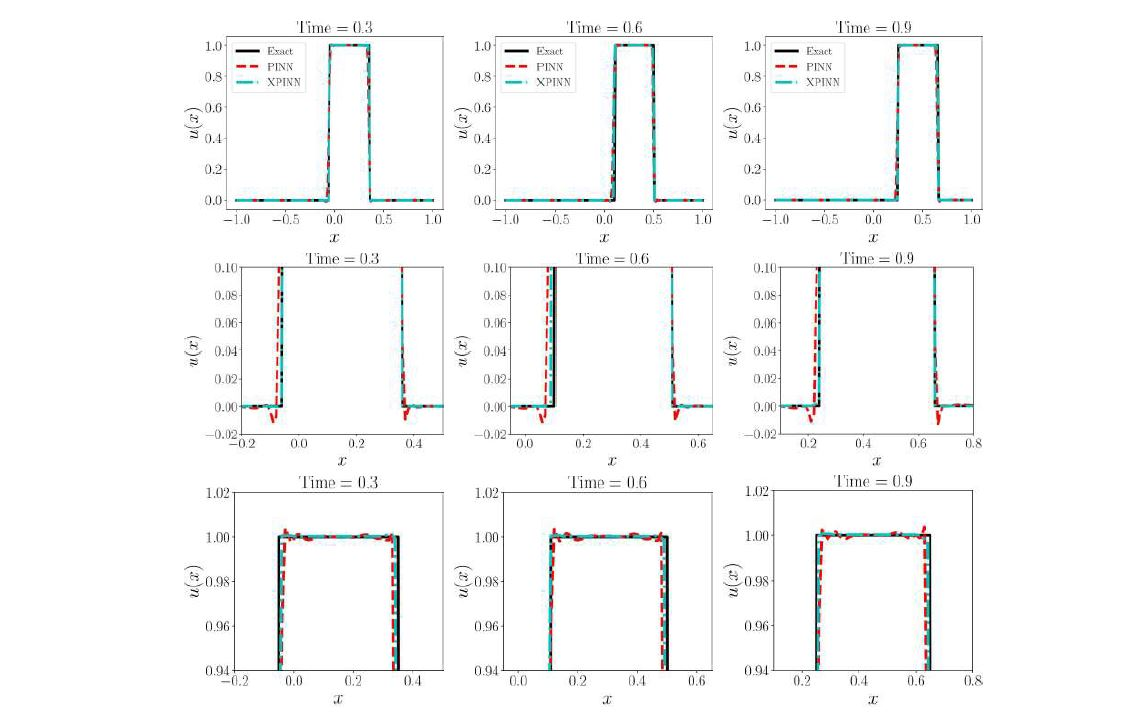
\includegraphics[scale=0.7]{figures/xpinn_result.JPG}
    \caption{Linear Advection Equation: Results for PINN and XPINN\cite{jagtap2020extended}}
\end{figure*}

According to the first, second, and third columns, the results for PINN and XPINN at different periods are shown in Figure 4\cite{jagtap2020extended}. whereas the second and third rows offer a zoomed-in perspective of the solutions, the first row shows the solution over a large area of space. XPINN's inference accuracy (relative L2 error is 6.0245e-2) is better than PINN's (relative L2 error 9.6589e-2)\cite{jagtap2020extended}. Due to the use of localized neural networks in the subdomain of XPINN rather than global networks in PINN, this is a significant improvement\cite{jagtap2020conservative}\cite{jagtap2020extended}.



\subsection{Bayesian-PINNs}


\begin{figure}[h]
    \centering
    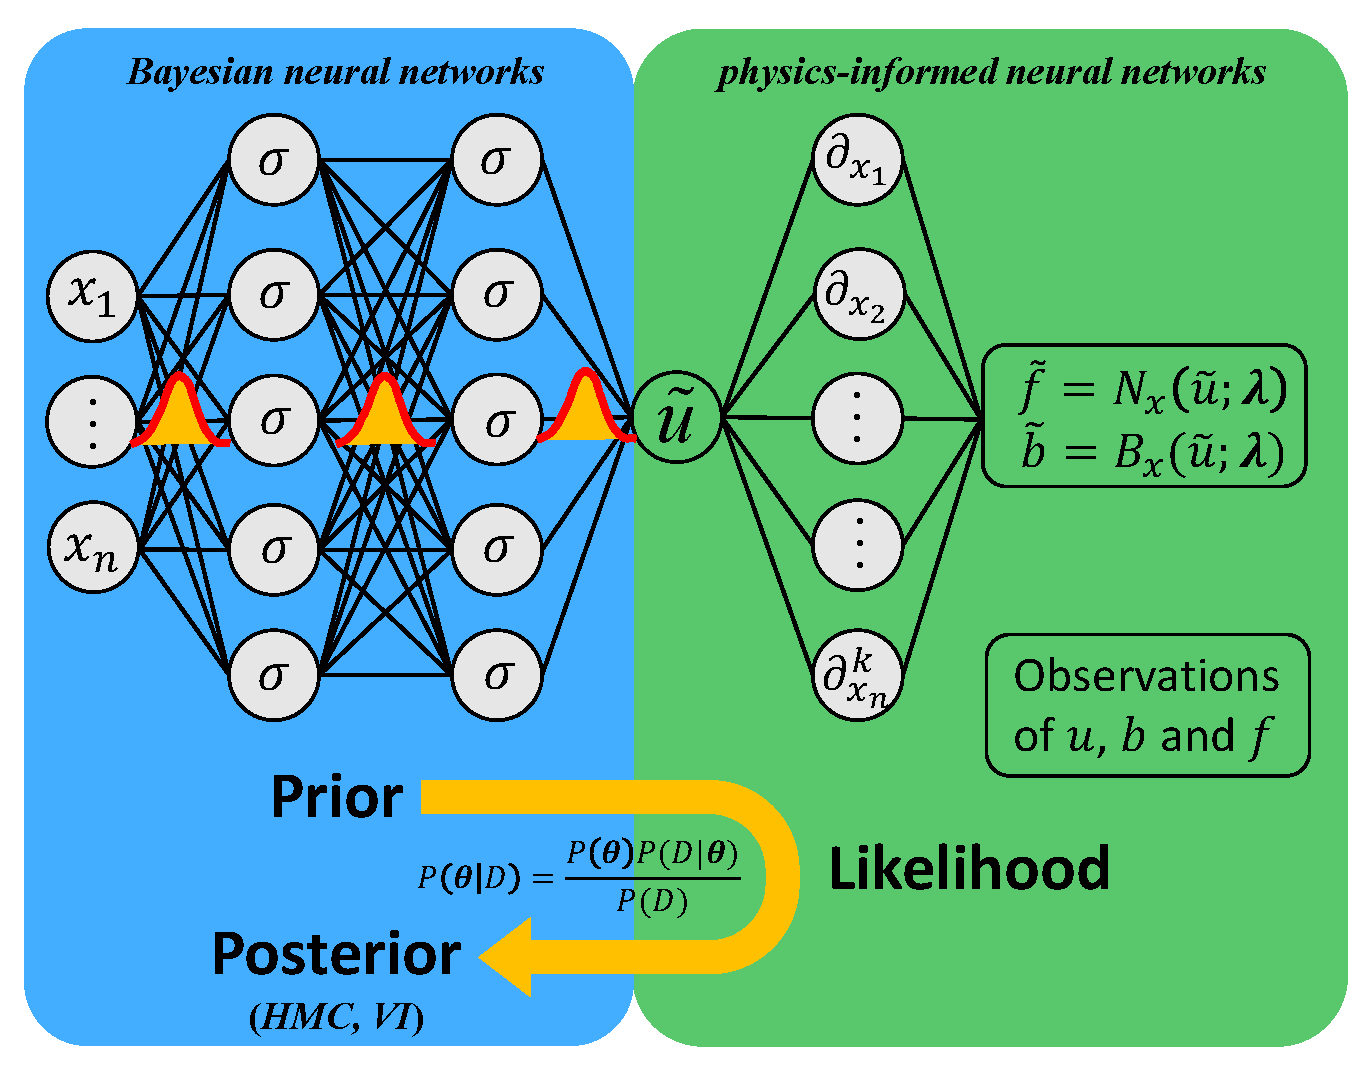
\includegraphics[scale=0.5]{figures/B-PINNs.png}
    \caption{Schematic for the Bayesian physics-informed neural network (B-PINN). $P(\theta)$ is the prior for hyperparameters as well as the unknown terms in  PDEs, $P\left(\mathcal{D}|\theta \right)$ represents the likelihood of observations (e.g., $u,\approx b, \approx f$), and $P(\theta|\mathcal{D})$ is the posterior. The blue panel represents the Bayesian neural network while the green panel represents the physics-informed part. \cite{yang2021b}}
    \label{fig:B-PINNs}
\end{figure}

Gaussian Process Regression (GPR) for PDEs and physics-informed neural networks (PINNs) are two common techniques to data driven modelling\cite{yang2021b}. Data-driven GPR is based on Bayesian framework with built-in uncertainty quantification mechanism\cite{zhang2019quantifying}. However, when used to solve PDEs, vanilla GPR has difficulty addressing non-linearities, resulting in limited applicability. As an alternative, PINNs for a wide range of PDEs have proven successful in both forward and inverse issues\cite{kharazmi2019variational}\cite{raissi2019physics}. There is no built-in uncertainty quantification in PINNs, however, which may limit their applicability, particularly in circumstances where the data is noisy.


To solve linear or nonlinear PDEs with scattered noisy data, (see Figure 5), the uncertainties originating from the scattered noisy data could be intrinsically quantified owing to Bayesian framework\cite{yang2021b}\cite{kharazmi2019variational}. BPINN is made out of two parts: a  parameterized  surrogate  model,  i.e.,  a  Bayesian neural  network  (BNN)  with  prior  for  the  unknown  terms  in  a  PDE,  and  an  approach for estimating the posterior distributions of the parameters in the surrogate model\cite{yang2021b}. Prior distributions were estimated using Hamiltonian Monte Carlo (HMC) [15, 16] and variational inference (VI) models\cite{kharazmi2019variational}.

%%%%%%%%%%%%%%%%%%%%%%%%%%%%%%%%%

%%%%%%%%%%%%%%%%%%%%%%%%%%%%%%%%%%



\subsubsection{Working}

Consider a general partial differential equation (PDE)  of the form 
\begin{equation}
\begin{aligned}
    \mathcal{N}_{\boldsymbol{x}}(u;\boldsymbol{\lambda}) &= f, \quad \boldsymbol{x}\in D, \\
    \mathcal{B}_{\boldsymbol{x}}(u;\boldsymbol{\lambda}) & = b, \quad \boldsymbol{x} \in \Gamma,
\end{aligned}
\end{equation}
where $\mathcal{N}_{\boldsymbol{x}}$ is a general differential operator, $D$ is the $d$-dimensional physical domain, $u = u(x)$ is the solution of the PDE, and $\boldsymbol{\lambda}$ is the vector of parameters in the PDE\cite{yang2021b}. 
Also, $f = f(x)$ is the forcing term, and $\mathcal{B}_{\boldsymbol{x}}$ is the boundary condition operator acting on the domain boundary $\Gamma$. In forward problems $\boldsymbol{\lambda}$ is prescribed, and hence the goal is to infer the distribution of $u$ at any $\boldsymbol{x}$. In inverse problems, $\boldsymbol{\lambda}$ is also to be inferred from the data\cite{yang2021b}\cite{xu2019neural}.


Consider the scenario where available dataset $\mathcal{D}$ are scattered noisy measurements of $u$, $f$ and $b$ from sensors:
\begin{equation}
    \begin{aligned}
    \mathcal{D} & = \mathcal{D}_u\cup\mathcal{D}_f\cup\mathcal{D}_b,
        \end{aligned}
\end{equation}
where,
\begin{align}
    \mathcal{D}_u = \{(\boldsymbol{x}_{u}^{(i)}, \bar{u}^{(i)})\}_{i=1}^{N_u}, \\
    \mathcal{D}_f  = \{(\boldsymbol{x}_{f}^{(i)}, \bar{f}^{(i)})\}_{i=1}^{N_f}, \\
    \mathcal{D}_b = \{(\boldsymbol{x}_{b}^{(i)}, \bar{b}^{(i)})\}_{i=1}^{N_b} \\
\end{align}

It was assumed that the measurements were independently Gaussian distributed centered at the hidden real value, i.e.,
\begin{equation}
    \begin{aligned}
    \bar{u}^{(i)} &= u(\boldsymbol{x}_{u}^{(i)}) + \epsilon_u^{(i)}, \quad i = 1,2...N_u, \\
    \bar{f}^{(i)} &= f(\boldsymbol{x}_{f}^{(i)}) + \epsilon_f^{(i)}, \quad i = 1,2...N_f, \\
    \bar{b}^{(i)} &= b(\boldsymbol{x}_{b}^{(i)}) + \epsilon_b^{(i)}, \quad i = 1,2...N_b,
    \end{aligned}
\end{equation}
where $\epsilon_u^{(i)}$, $\epsilon_f^{(i)}$ and $\epsilon_b^{(i)}$ are independent Gaussian noises with zero mean. It is also assumed that the fidelity of each sensor is known\cite{raissi2017inferring}, i.e., the standard deviations of $\epsilon_u^{(i)}$, $\epsilon_f^{(i)}$ and $\epsilon_b^{(i)}$ are known to be $\sigma_u^{(i)}$, $\sigma_f^{(i)}$ and $\sigma_b^{(i)}$, respectively. Note that the size of the noise could be different among measurements of different terms, and even between measurements of the same terms in the PDE.



In the {\em forward} problem setup, the Bayesian framework starts from representing $u$ with a surrogate model $\tilde{u}(\boldsymbol{x}; \boldsymbol{\theta})$, where $\boldsymbol{\theta}$ is the vector of parameters in the surrogate model with a prior distribution $P(\boldsymbol{\theta})$. Consequently, $f$ and $b$ are represented by: 
\begin{equation}
\label{eqn:fb}
\begin{aligned}
    \tilde{f}(\boldsymbol{x}; \boldsymbol{\theta}) = \mathcal{N}_{\boldsymbol{x}}(\tilde{u}(\boldsymbol{x}; \boldsymbol{\theta});\boldsymbol{\lambda}), ~\tilde{b}(\boldsymbol{x}; \boldsymbol{\theta}) = \mathcal{B}_{\boldsymbol{x}}(\tilde{u}(\boldsymbol{x}; \boldsymbol{\theta}) ;\boldsymbol{\lambda}).
\end{aligned}
\end{equation}
\newline
Then, the likelihood can be calculated as:
\begin{equation}
\label{eqn:likelihood}
\begin{aligned}
    P(\mathcal{D}|\boldsymbol{\theta}) &= P(\mathcal{D}_u|\boldsymbol{\theta}) P(\mathcal{D}_f|\boldsymbol{\theta}) P(\mathcal{D}_b|\boldsymbol{\theta}), \\
     P(\mathcal{D}_u|\boldsymbol{\theta}) &= \prod_{i=1}^{N_u} \frac{1}{\sqrt{2\pi{\sigma_u^{(i)}}^2}}\exp \left(-\frac{(\tilde{u}(\boldsymbol{x}_{u}^{(i)}; \boldsymbol{\theta}) - \bar{u}^{(i)})^2}{2{\sigma_u^{(i)}}^2}\right), \\
     P(\mathcal{D}_f|\boldsymbol{\theta}) &= \prod_{i=1}^{N_f} \frac{1}{\sqrt{2\pi{\sigma_f^{(i)}}^2}}\exp \left(-\frac{(\tilde{f}(\boldsymbol{x}_{f}^{(i)}; \boldsymbol{\theta}) - \bar{f}^{(i)})^2}{2{\sigma_f^{(i)}}^2}\right), \\
    P(\mathcal{D}_b|\boldsymbol{\theta}) &= \prod_{i=1}^{N_b} \frac{1}{\sqrt{2\pi{\sigma_b^{(i)}}^2}}\exp \left(-\frac{(\tilde{b}(\boldsymbol{x}_{b}^{(i)}; \boldsymbol{\theta}) - \bar{b}^{(i)})^2}{2{\sigma_b^{(i)}}^2}\right). \\
\end{aligned}
\end{equation}
Finally, the posterior is obtained from Bayes' theorem:
\begin{equation}
\label{eqn:forwardpost}
\begin{aligned}
P(\boldsymbol{\theta}| \mathcal{D}) = \frac{ P(\mathcal{D}|\boldsymbol{\theta})P(\boldsymbol{\theta})}{P(\mathcal{D})} \simeq P(\mathcal{D}|\boldsymbol{\theta})P(\boldsymbol{\theta}),
\end{aligned}
\end{equation}
where ``$\simeq$'' represents equality up to a constant. To give a posterior $u$ at any $\boldsymbol{x}$, sample from $P(\boldsymbol{\theta}| \mathcal{D})$ can be obtained, denoted as $\{{\boldsymbol{\theta}}^{(i)}\}_{i=1}^M$, and then obtain statistics from samples $\{\tilde{u}(\boldsymbol{x}; {\boldsymbol{\theta}}^{(i)} ) \}_{i=1}^M$. The focus is mostly on the mean and standard deviation of $\{\tilde{u}(\boldsymbol{x}; {\boldsymbol{\theta}}^{(i)} ) \}_{i=1}^M$, since the former represents the prediction of  $u(\boldsymbol{x})$ while the latter quantifies the uncertainty.

In the case of inverse problems, surrogate model for $u$ can be built\cite{lou2020physics}\cite{yang2021b}. However, apart from $\boldsymbol{\theta}$, assignment of a prior distribution for $\boldsymbol{\lambda}$ is also required, which could be independent of $P(\boldsymbol{\theta})$. The likelihood is the same as in Eq.~\ref{eqn:likelihood}, except that $P(\mathcal{D}|\boldsymbol{\theta})$, $P(\mathcal{D}_u|\boldsymbol{\theta})$, $P(\mathcal{D}_f|\boldsymbol{\theta})$ and $P(\mathcal{D}_b|\boldsymbol{\theta})$ should be replaced by 
$P(\mathcal{D}|\boldsymbol{\theta},\boldsymbol{\lambda})$, $P(\mathcal{D}_u|\boldsymbol{\theta},\boldsymbol{\lambda})$, $P(\mathcal{D}_f|\boldsymbol{\theta},\boldsymbol{\lambda})$ and $P(\mathcal{D}_b|\boldsymbol{\theta},\boldsymbol{\lambda})$, respectively.  Consequently, joint posterior of $[\boldsymbol{\theta}, \boldsymbol{\lambda}]$ can be calculated as
\begin{equation}
\label{eqn:backwardpost}
\begin{aligned}
P(\boldsymbol{\theta}, \boldsymbol{\lambda} | \mathcal{D}) = \frac{ P(\mathcal{D}|\boldsymbol{\theta},\boldsymbol{\lambda})P(\boldsymbol{\theta},\boldsymbol{\lambda})}{P(\mathcal{D})} \\ \simeq P(\mathcal{D}|\boldsymbol{\theta},\boldsymbol{\lambda})P(\boldsymbol{\theta},\boldsymbol{\lambda}) = P(\mathcal{D}|\boldsymbol{\theta},\boldsymbol{\lambda})P(\boldsymbol{\theta})P(\boldsymbol{\lambda}),
\end{aligned}
\end{equation}
where the last equality comes from the fact that the priors for $\boldsymbol{\theta}$ and $\boldsymbol{\lambda}$ are independent.

The parameter $\boldsymbol{\lambda}$ in the PDE is a vector in the above problem setup, however, the same framework could be applied in the cases where the parameter is a field or fields depending on $\boldsymbol{x}$, by representing the parameter vector with another surrogate model\cite{yang2021b}.

Since the forward problems and inverse problems are formulated in the same framework, $\boldsymbol{\theta}$ is used to represent the vector of all the unknown parameters in the surrogate models for the solutions and parameters\cite{lou2020physics}\cite{yang2021b}. The dimension of $\boldsymbol{\theta}$, i.e., the number of unknown parameters,are denoted as $d_{\boldsymbol{\theta}}$. 



\subsubsection{Results}

Consider the following 1D nonlinear PDE
\begin{align}\label{eq:nonlinear}
    \lambda \partial^2_x u + k \tanh(u) = f , x \in [-0.7, 0.7],
\end{align}

The objective here is to identify k based on partial measurements of f and u.

\begin{figure}
    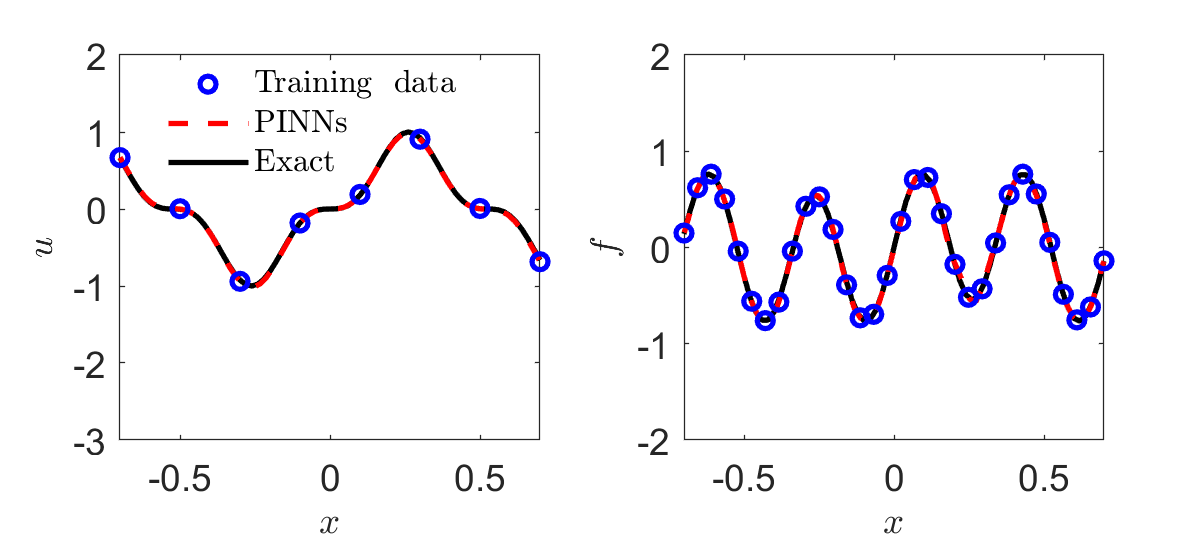
\includegraphics[width=0.45\textwidth]{figures/1D_inverse_pinn_001.png}
    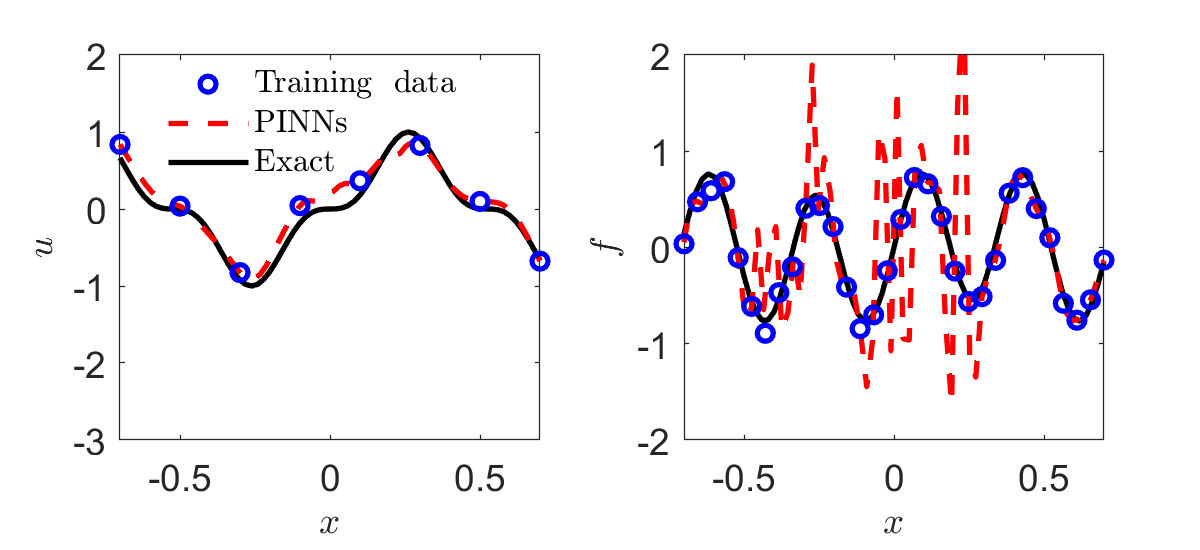
\includegraphics[width=0.45\textwidth]{figures/1D_inverse_pinn_01.png}
    \caption{1D diffusion-reaction system with nonlinear source term (PINNs): Predicted $u$ and $f$ with two data noise scales.
        (a) $\epsilon_f \mathcal{N}(0, 0.01^2)$, $\epsilon_u  \mathcal{N}(0, 0.01^2)$, $\epsilon_b  \mathcal{N}(0, 0.01^2)$. 
        (b) $\epsilon_f  \mathcal{N}(0, 0.1^2)$, $\epsilon_u  \mathcal{N}(0, 0.01^2)$, $\epsilon_b                                \mathcal{N}(0,0.1^2)$\cite{yang2021b}.}
    \label{fig:pinninverse}
\end{figure}


\begin{figure*}
    \centering
    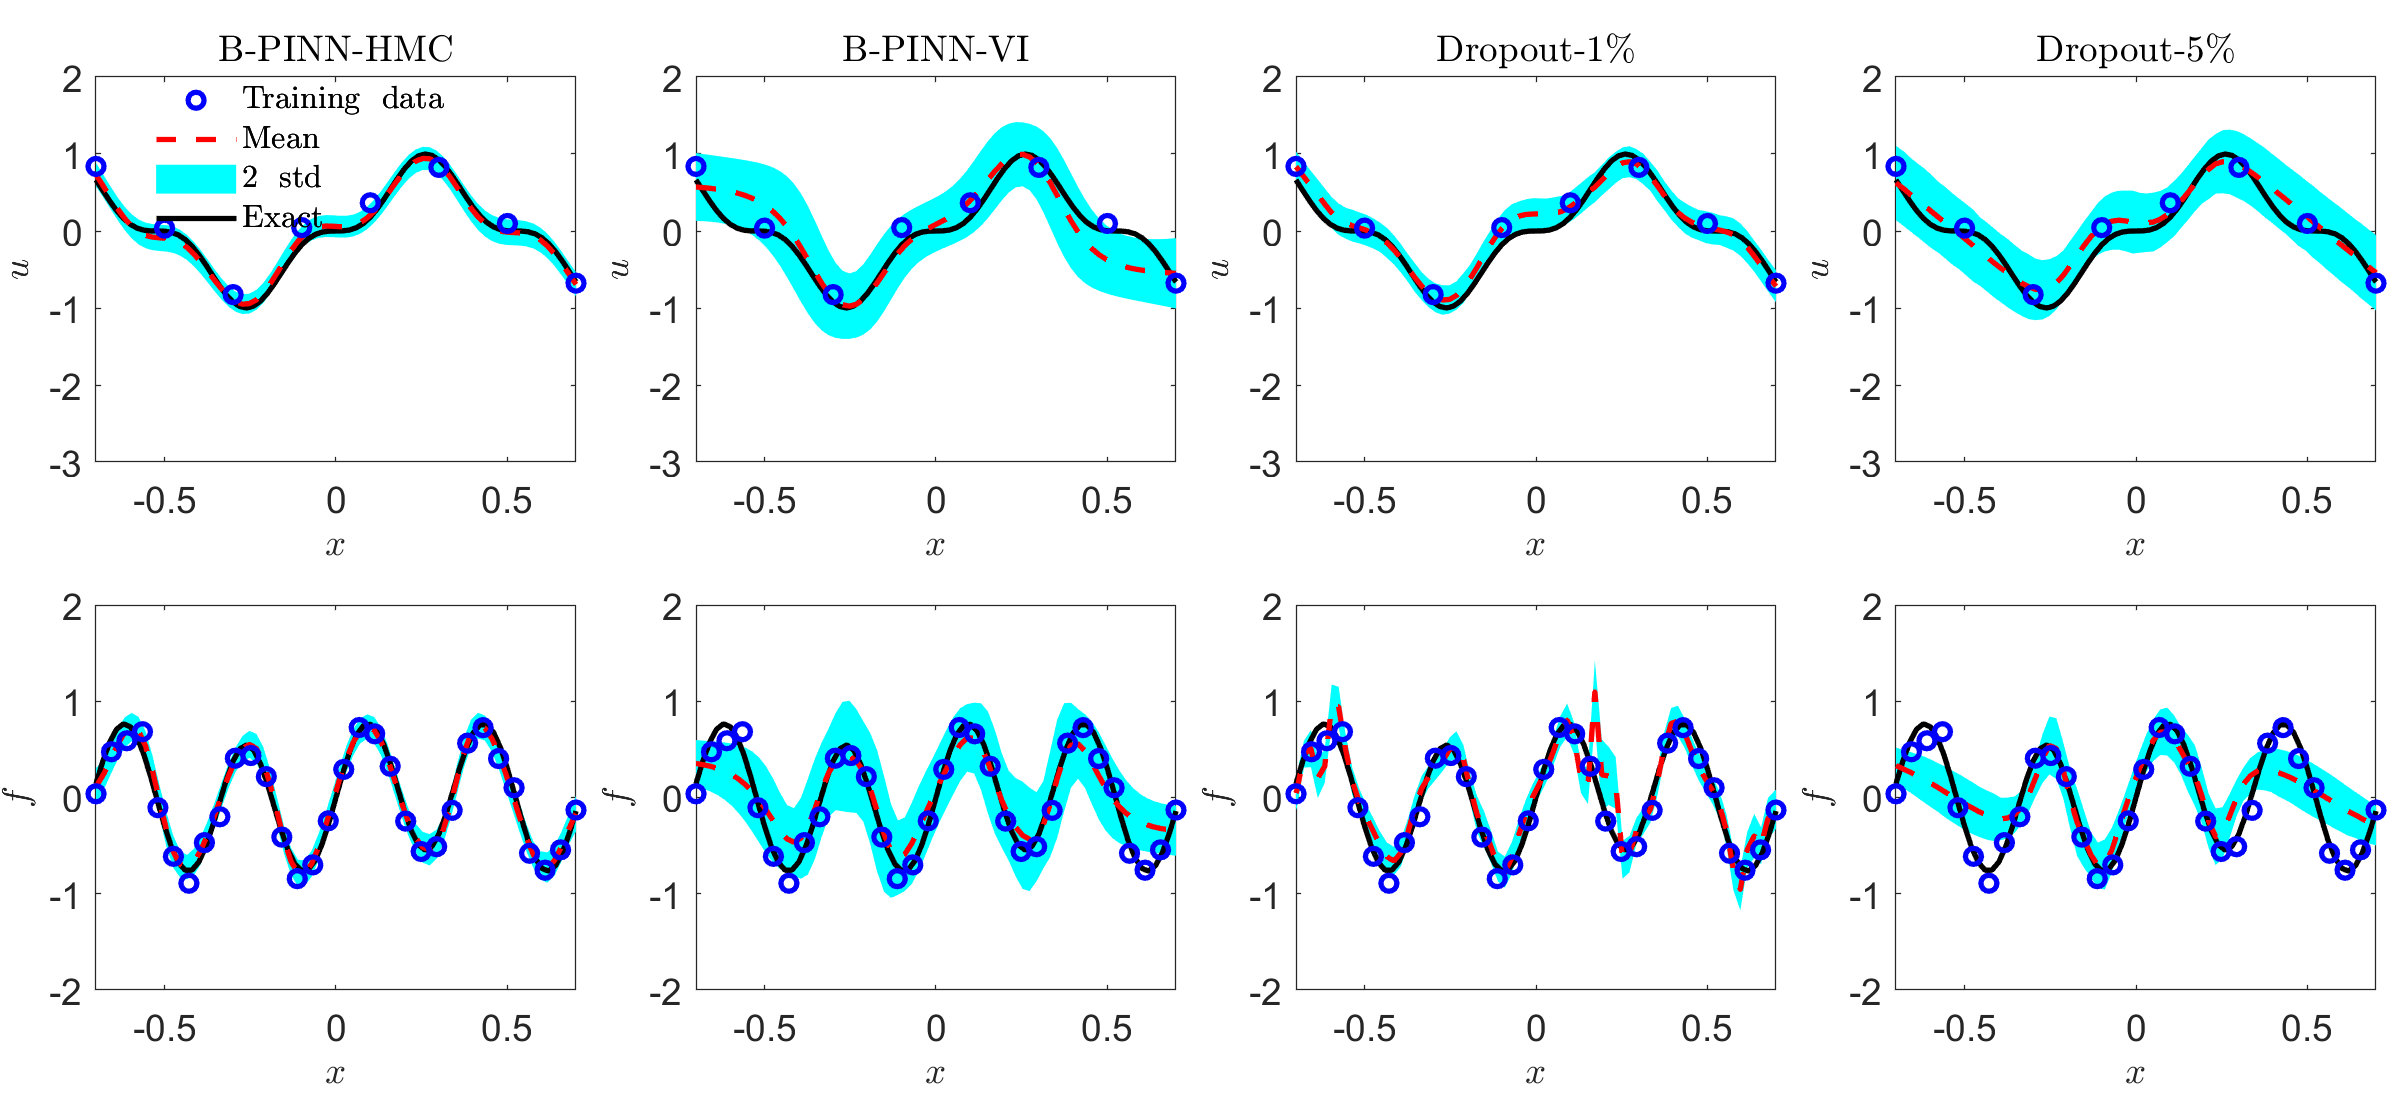
\includegraphics[scale=0.25]{figures/1D_nonlinear_inverse_BNN_01.png}
    \caption{1D diffusion-reaction system with nonlinear source term - inverse problem: predicted $u$ and $f$ from different methods with noisy data. $\epsilon_f  \mathcal{N}(0, 0.1^2)$, $\epsilon_u  \mathcal{N}(0, 0.1^2)$, $\epsilon_b  \mathcal{N}(0, 0.01^2)$.\cite{yang2021b}}
\end{figure*}

As shown in Fig.6, the predicted $u$ and $f$ could fit all the training points. In the cases where the noise scale is as small as $0.01$, the predictive $u$ and $f$ agree well with the exact solutions. However, as the noise scale increases to 0.1, significant overfitting is observed in PINNs\cite{raissi2019physics}. In addition, PINNs predict $k$ to be $0.705$ and $0.591$ for the noise lebel at $0.01$ and $0.1$, respectively, while the reference exact solution is $0.7$\cite{yang2021b}. Comparing with the results of B-PINN in Fig.7, it can be concluded that PINNs can provide prediction with similar accuracy as the B-PINN-HMC for the case with small noise in data, while B-PINN-HMC shows significant advantange in accuracy over  PINNs for the case with large noise\cite{yang2021b}.



\subsection{PI-GANs}

GANs can be used to represent physical and biological systems with intrinsic stochasticity and extrinsic uncertainty\cite{yang2018physics}\cite{cai2021physics}. Although physics-informed neural networks were initially proposed in [12, 13], work that has directly encoded known physical principles into GAN frameworks was not found\cite{yang2018physics}.

The goal is to use GANs to model and learn unknown stochastic variables from data while embedding the known physics, especially the form of the stochastic differential equation (SDE)\cite{yang2020generative}. To do this, models and data were used to make both inferences and system identifications\cite{yang2018physics}. This method was used for the mixed situations, where enough evidence is not present for either but want to infer both states and systems\cite{yang2018physics}.



%%%%%%%%%%Review SDEs%%%%%%%%%%%

However, the majority of published papers deal with deterministic systems. Although there are very few studies published on data-driven techniques for SDEs for forward problems. When modeling stochastic systems in high dimensions, this approach suffers from the "curse of dimensionality," which is a phenomenon where the number of polynomial chaotic expansion terms grows exponentially as the effective dimension increases.

\begin{figure}
    \centering
    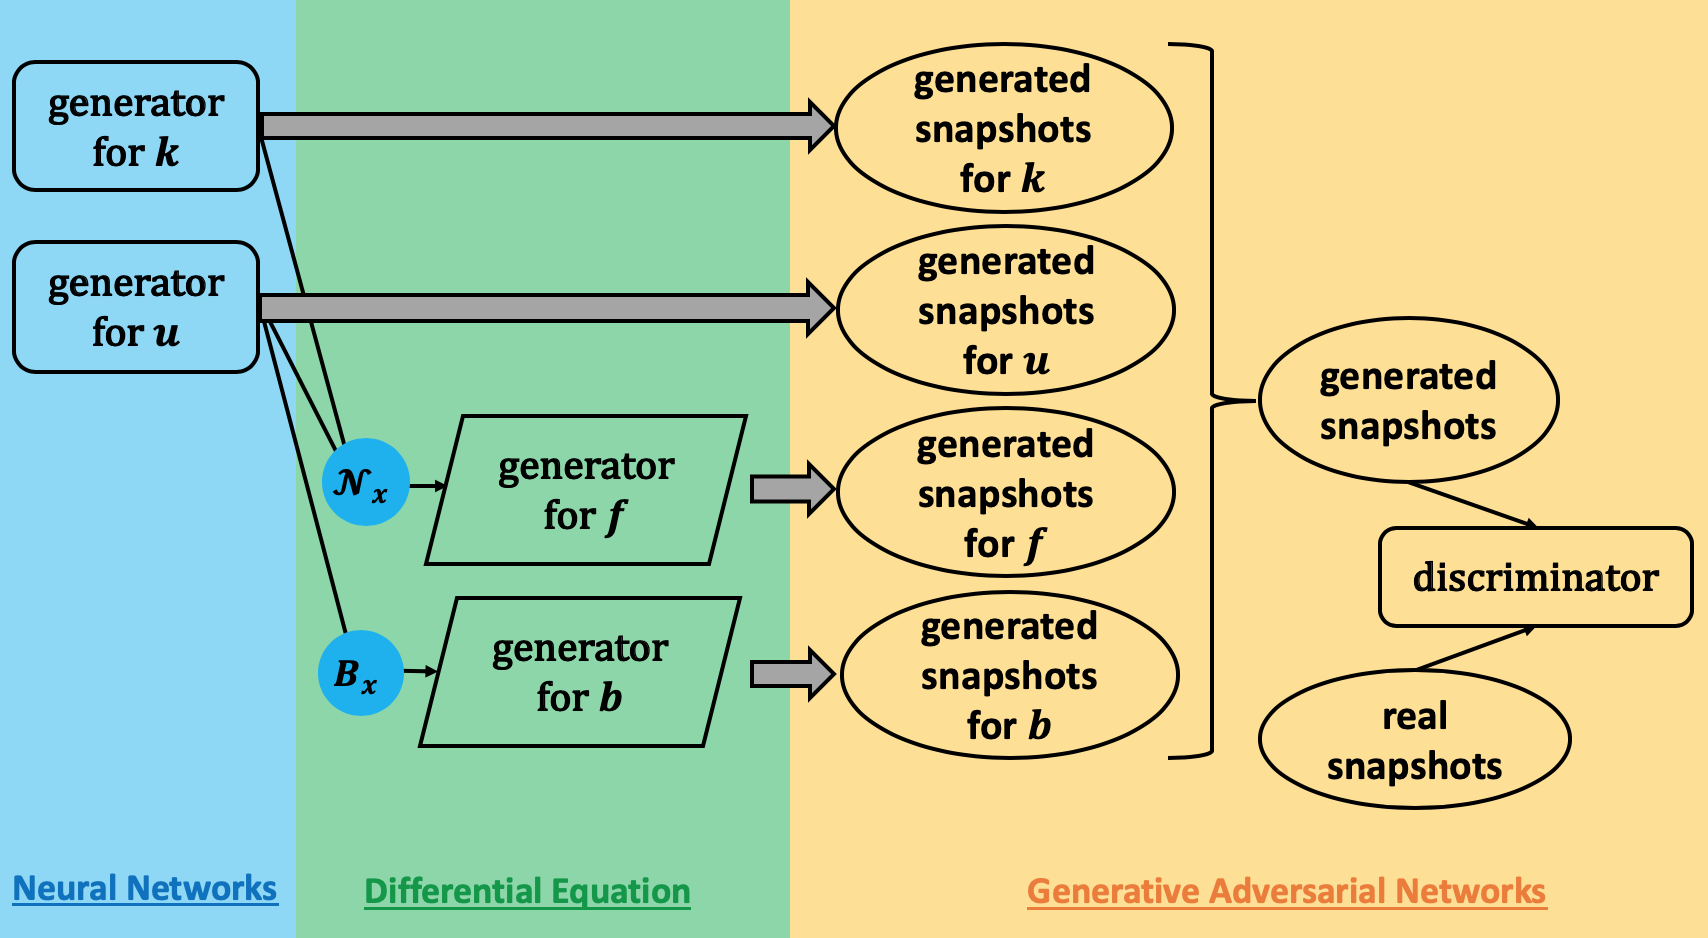
\includegraphics[scale=0.25]{figures/PIGAN.png}
    \caption{PIGAN architecture\cite{yang2018physics}}
\end{figure}


%%%%%%%%%%Finally%%%%%%%%%%%
GANs that are trained on physical data may be used for addressing a wide range of SDE issues, from forward to inverse problems, and everything in between\cite{yang2018physics}\cite{lou2020physics}. To make matters even better, PI-GANs avoid the "curse of dimension". Because of this, it is possible for SDEs that include stochastic processes to be solved by PI-GANs\cite{yang2018physics}.


\subsubsection{Working}

As a pedagogical problem, let us first consider the problem of modeling a stochastic process $f(x;\omega)$ on the domain $D \in \mathbb{R}^d$ with GANs\cite{yang2018physics}. The total $N$ snapshots of $f(x;\omega)$ sensor data is usd as the training set:
\begin{equation}
    \{F(\omega^{(j)})\}_{j=1}^N = \{(f(x_i;\omega^{(j)}))_{i=1}^{n} \}_{j=1}^N,
\end{equation}
where $n$ is the number of sensors and $\{x_i\}_{i=1}^n$ are positions of the sensors. Feed forward DNN $\tilde{f}_{\theta}(x;\boldsymbol{\xi})$ parameterized by $\theta$ is used as the generator to model the stochastic process $f(x;\omega)$. The generator takes the concatenation of a noise vector $\boldsymbol{\xi} \sim Q_z$ from $\mathbb{R}^{m}$ and the coordinate $x$ as the input, while the output is a real number representing $\tilde{f}_{\theta}(x;\boldsymbol{\xi})$. Let
\begin{equation}
    \{\tilde{F}(\boldsymbol{\xi}^{(j)})\}_{j} = \{(\tilde{f}_{\theta}(x_i;\boldsymbol{\xi}^{(j)}))_{i=1}^{n}\}_{j}
\end{equation}
be the generated ``fake'' snapshots, where $\{\boldsymbol{\xi}^{(j)} \}_{j}$ are instances of $\boldsymbol{\xi}$ with $j$ as the index.

The discriminator $D_{\rho}(\cdot)$ is implemented as another feed forward DNN parameterized by $\rho$. The GAN strategy shall be applied by feeding both the real and generated snapshots into the discriminator, and train the generator and discriminator iteratively\cite{yang2018physics}.

PI-GANs consists of the following three steps:

First, two independent feed forward DNNs are used, namely $\tilde{k}_{\theta_k}(x;\boldsymbol{\xi} )$ and $\tilde{u}_{\theta_u}(x;\boldsymbol{\xi} )$ parameterized by $\theta_k$ and $\theta_u$, to represent the stochastic processes $k(x;\omega)$ and $u(x;\omega)$ in the aforementioned way.

Second, inspired by the physics-informed neural networks for deterministic PDEs\cite{yang2018physics}, the equation are encoded into the neural networks system by applying the operator $\mathcal{N}_x$ and $B_x$ on the feed forward DNNs $\tilde{k}_{\theta_k}(x;\boldsymbol{\xi} )$ and $\tilde{u}_{\theta_u}(x;\boldsymbol{\xi} )$ to generate ``induced'' neural networks, which are formulated as
\begin{equation} 
\tilde{f}_{\theta_u, \theta_k}(x;\boldsymbol{\xi}) = \mathcal{N}_x [\tilde{u}_{\theta_u}(x;\boldsymbol{\xi}); \tilde{k}_{\theta_k}(x;\boldsymbol{\xi})]
\end{equation}
and 
\begin{equation} 
\tilde{b}_{\theta_u}(x;\boldsymbol{\xi}) =B_x[\tilde{u}_{\theta_u}(x;\boldsymbol{\xi})].
\end{equation}

Differentiation in $\mathcal{N}_x$ and $B_x$ are performed by automatic differentiation~\cite{baydin2018automatic}. $\tilde{f}_{\theta_u, \theta_k}(x;\boldsymbol{\xi})$ and $\tilde{b}_{\theta_u}(x;\boldsymbol{\xi})$ are used as the generators of $f(x;\omega)$ and $b(x;\omega)$, respectively. Note that both $\tilde{f}_{\theta_u, \theta_k}(x;\boldsymbol{\xi})$ and $\tilde{b}_{\theta_u}(x;\boldsymbol{\xi})$ are induced from $\tilde{u}_{\theta_u}(x;\boldsymbol{\xi})$ and $\tilde{k}_{\theta_k}(x;\boldsymbol{\xi})$, thus the parameters $\theta_k$ and $\theta_u$ are directly inherited from $\tilde{u}$ and $\tilde{k}$.



In the third step, training data is incorporated to conduct adversarial training. The training data are collected as a group of snapshots. The corresponding generated ``fake'' snapshots are
\begin{equation} \label{eqn:G}
\begin{aligned}
\{G(\boldsymbol{\xi}^{(j)})\}_j & = \{(\tilde{K}(\boldsymbol{\xi}^{(j)}), \tilde{U}(\boldsymbol{\xi}^{(j)}),\tilde{F}(\boldsymbol{\xi}^{(j)}),\tilde{B}(\boldsymbol{\xi}^{(j)}))\}_j,\\
\tilde{K}(\boldsymbol{\xi}^{(j)}) & = (\tilde{k}_{\theta_k}(x_i^k;\boldsymbol{\xi}^{(j)}))_{i=1}^{n_k},\\
\tilde{U}(\boldsymbol{\xi}^{(j)}) & = (\tilde{u}_{\theta_u}(x_i^u;\boldsymbol{\xi}^{(j)}))_{i=1}^{n_u},\\
\tilde{F}(\boldsymbol{\xi}^{(j)}) & = (\tilde{f}_{\theta_k,\theta_u}(x_i^f;\boldsymbol{\xi}^{(j)}))_{i=1}^{n_f},\\
\tilde{B}(\boldsymbol{\xi}^{(j)}) & = (\tilde{b}_{\theta_u}(x_i^b;\boldsymbol{\xi}^{(j)}))_{i=1}^{n_b},
\end{aligned}
\end{equation}
where $\{\boldsymbol{\xi}^{(j)} \}_{j}$ are instances of $\boldsymbol{\xi}$ with $j$ as the index. The generated snapshots and real snapshots could be then fed into discriminator, and train the generators and discriminators iteratively \cite{yang2018physics}. With well trained generators, all the data can be predicted with sample paths created by the generators.


If the snapshots are collected in $M$ groups ($M>1$), groups of $M$ ``fake'' snapshots also need to be generated:
\begin{equation} \label{eqn:G_multi}
\begin{aligned}
\{\{G_t(\boldsymbol{\xi}^{(t,j)}\}_j\}_{t=1}^M & = \{\{(\tilde{K_t}(\boldsymbol{\xi}^{(t,j)}), \tilde{U_t}(\boldsymbol{\xi}^{(t,j)}),\\ \tilde{F_t}(\boldsymbol{\xi}^{(t,j)}),\tilde{B_t}(\boldsymbol{\xi}^{(t,j)}))\}_j\}_{t=1}^{M},\\
\tilde{K_t}(\boldsymbol{\xi}^{(t,j)}) & = (\tilde{k}_{\theta_k}(x_i^{k,t};\boldsymbol{\xi}^{(t,j)}))_{i=1}^{n_{k,t}},\\
\tilde{U_t}(\boldsymbol{\xi}^{(t,j)}) & = (\tilde{u}_{\theta_u}(x_i^{u,t};\boldsymbol{\xi}^{(t,j)}))_{i=1}^{n_{u,t}},\\
\tilde{F_t}(\boldsymbol{\xi}^{(t,j)}) & = (\tilde{f}_{\theta_k,\theta_u}(x_i^{f,t};\boldsymbol{\xi}^{(t,j)}))_{i=1}^{n_{f,t}},\\
\tilde{B_t}(\boldsymbol{\xi}^{(t,j)}) & = (\tilde{b}_{\theta_u}(x_i^{b,t};\boldsymbol{\xi}^{(t,j)}))_{i=1}^{n_{b,t}},\\
\end{aligned}
\end{equation}
where $t$s are the indices for the groups, $\boldsymbol{\xi}^{(t,j)}$ is an instance of $\boldsymbol{\xi}$ for each $(t,j)$, $\{x^{k,t}_i\}_{i=1}^{n_{k,t}}$ is the position setup of $n_{k,t}$ sensors for $k$ in group $t$ (similarly for other terms). 
%
Multiple discriminators were used $\{D_{\rho_t}(\cdot)\}_t^M$, with each discriminator focusing on one group of snapshots, while the generators need to ``deceive'' all the discriminators simultaneously\cite{yang2018physics}. 

For the case where only one group of data is available, set $M = 1$ . For simplicity, here the weight were set in the generator loss function $a_t = 1$ for each $t$, which works well, but the method of setting $\{a_t\}_{t=1}^M$ requires further study.


Note that the method does not explicitly distinguish the three types of problems\cite{yang2018physics}. Solving forward problems, inverse problems or mixed problems actually uses the same framework\cite{lou2020physics}.
 


\subsubsection{Results}

Consider the stochastic elliptic equation, and $k(x;\omega)$ and $f(x;\omega)$ as the following independent stochastic processes:
\begin{equation} \label{eqn:samples}
\begin{aligned}
	 k(x) & = \exp[\frac{1}{5}\sin(\frac{3\pi}{2}(x +1)) + \hat{k}(x)] \\
	\hat{k}(x) & \sim \mathcal{GP}\left(0, \frac{4}{25}\exp(-(x-x')^2)\right) \\
	f(x) & \sim \mathcal{GP}\left(\frac{1}{2}, \frac{9}{400}\exp(-25(x-x')^2)\right) \\
\end{aligned}
\end{equation}
In this case, 13 dimensions are needed to retain $99\%$ energy of $f(x;\omega)$. 13 $k$-sensors , 21 $f$-sensors and 2 $u$-sensors were used on the boundary of physical domain $\mathcal{D}$.

\begin{figure}
    \centering
    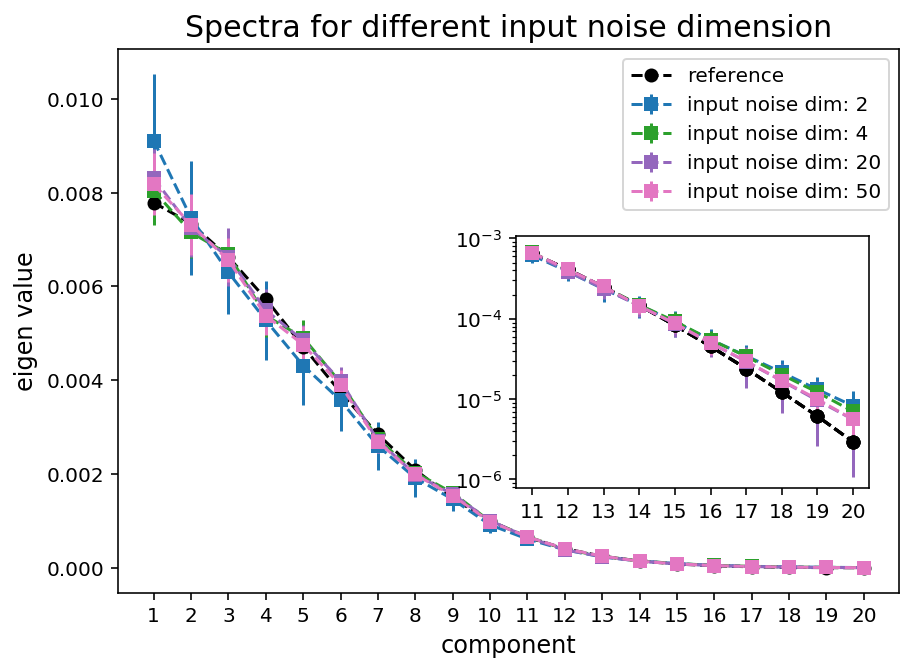
\includegraphics[scale=0.4]{figures/1_EigenValue_4.png}	
    \label{fig:1_PCA_1}
    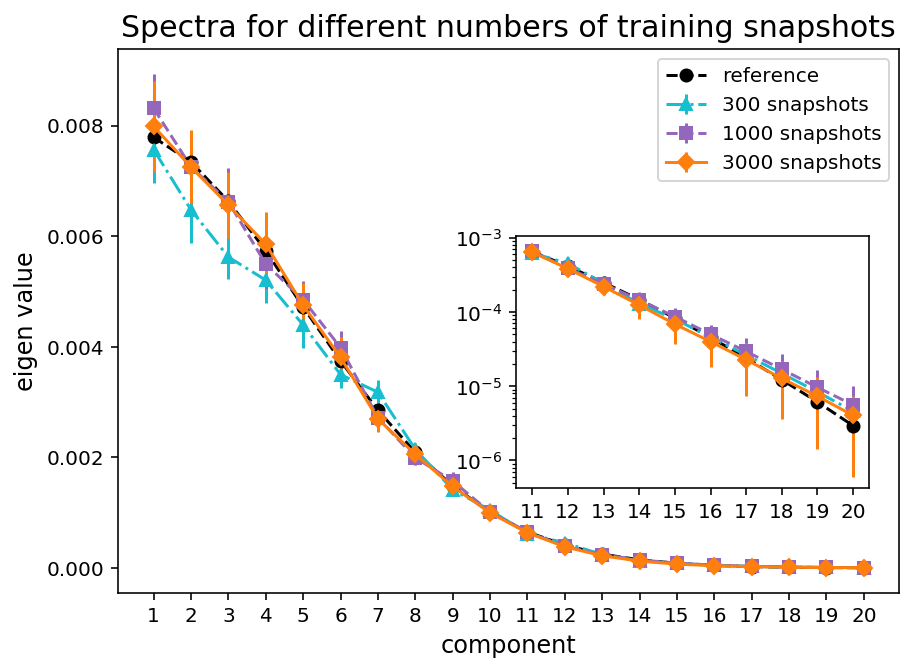
\includegraphics[scale=0.4]{figures/1_EigenValue_5.png}
    \label{fig:1_PCA_2}
	\caption{Forward problem: spectra of generated right-hand-side $f(x;\omega)$ processes. (a): Varying input noise dimension for a fixed number of snapshots at 1000. (b): Varying the number of training snapshots for a fixed dimension of input noise at 20. The inset plots are the zoom-ins of the eigenvalues of high frequency modes.  The means (markers) and two standard deviations (vertical lines on the markers) are calculated from the selected 33 generators. The reference curves are calculated from another $1\times 10^5$ independent $f(x;\omega)$ sample paths.\cite{yang2018physics}}
\end{figure}

To study the influence of input noise dimension, the number of training snapshots were fixed to be 1000, and vary the input noise dimension to be 2, 4, 20 and 50. Subsequently, input noise dimension was fixed as 20 and vary the number of training snapshots to be 300, 1000 and 3000 to study the influence of the number of training snapshots\cite{yang2018physics}.



The spectra of the generated processes for $f(x;\omega)$ is illustrated in Figure 9  to verify that the generated processes captured the covariance structure of $f(x;\omega)$. It can be seen that the spectra of generated processes fit the reference solution well. With fixed number of training snapshots, as input noise dimension is increased, the gap between generated processes and the reference solutions narrows\cite{zhu2019physics}. With fixed input noise dimension, the gap narrows as the number of training snapshots are increased. These observations on the spectra are similar with those about the error of $u$\cite{yang2018physics}.



\subsection{Parareal-PINNs}
Significant spatial-temporal degrees of freedom contribute to a large amount of data for training the PINN in situations involving long-time integration of PDEs\cite{meng2020ppinn}. These long-time physical problems may prove computationally expensive if PINNs are used\cite{cai2021physics}\cite{zhang2020learning}.
%
So, \emph{parareal physics-informed neural network} (PPINN) is proposed to break one long-time issue into several independent short-time problems under the supervision of an inexpensive/fast coarse grain solver (CG)\cite{meng2020ppinn}. In order to leverage the benefits of great computing efficiency while training a neural network, this PPINN architecture takes use of the fact that DNN training costs grow rapidly with data size. Specific benefits include the fact that training individual PINNs with smaller data sets is significantly faster than working directly with big data sets, and that training fine PINNs can be easily parallelized on several GPU-CPU cores\cite{meng2020ppinn}. For one-dimensional and two-dimensional nonlinear issues, the suggested PPINN technique may be more efficient than the original PINN approach in terms of tackling long-term physical difficulties\cite{cai2021physics}. However, a good supervisor will be required, which is represented by a coarse-grained (CG) solver that should be accurate\cite{meng2020ppinn}.

\begin{figure*}
  \centering
  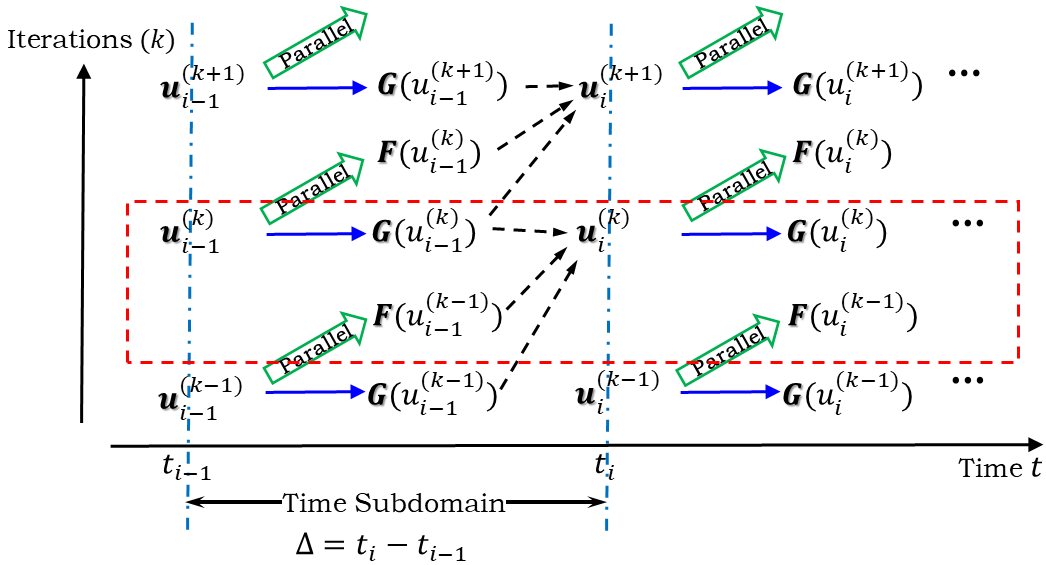
\includegraphics[scale=0.6]{figures/Figure2b.png}\\
  \caption{A graphical representation of the parallel-in-time algorithm used in PPINN, in which a cheap serial CG solver is used to make an approximate prediction of the solution $\mathcal{G}(\mathbf{u}_i^k)$, while many fine PINNs are performed in parallel for getting $\mathcal{F}(\mathbf{u}_i^k)$ to correct the solution iteratively. Here, $k$ represents the index of iteration, and $i$ is the index of time subdomain.\cite{meng2020ppinn}}
\end{figure*}

\subsubsection{Working}
For a time-dependent problem involving long-time integration of PDEs for $t\in [0,T]$, instead of solving this problem directly in one single time domain, PPINN splits $[0,T]$ into $N$ sub-domains with equal length $\Delta T = T/N$. Then, PPINN employs two propagators, i.e., a serial CG solver and $N$ fine PINNs computing in parallel\cite{meng2020ppinn}. Here, $\mathbf{u}_{i}^k$ denotes the approximation to the exact solution at time $t_i$ in the $k$-{th} iteration. Because the CG solver is serial in time and fine PINNs run in parallel, to have the optimal computational efficiency,a simplified PDE (sPDE) is encoded into the CG solver as a prediction propagator while the true PDE is encoded in fine PINNs as the correction propagator\cite{meng2020ppinn}.
Using this prediction-correction strategy, the PPINN solution is expected to converge to the true solution after a few iterations.


\begin{figure}
  \centering
  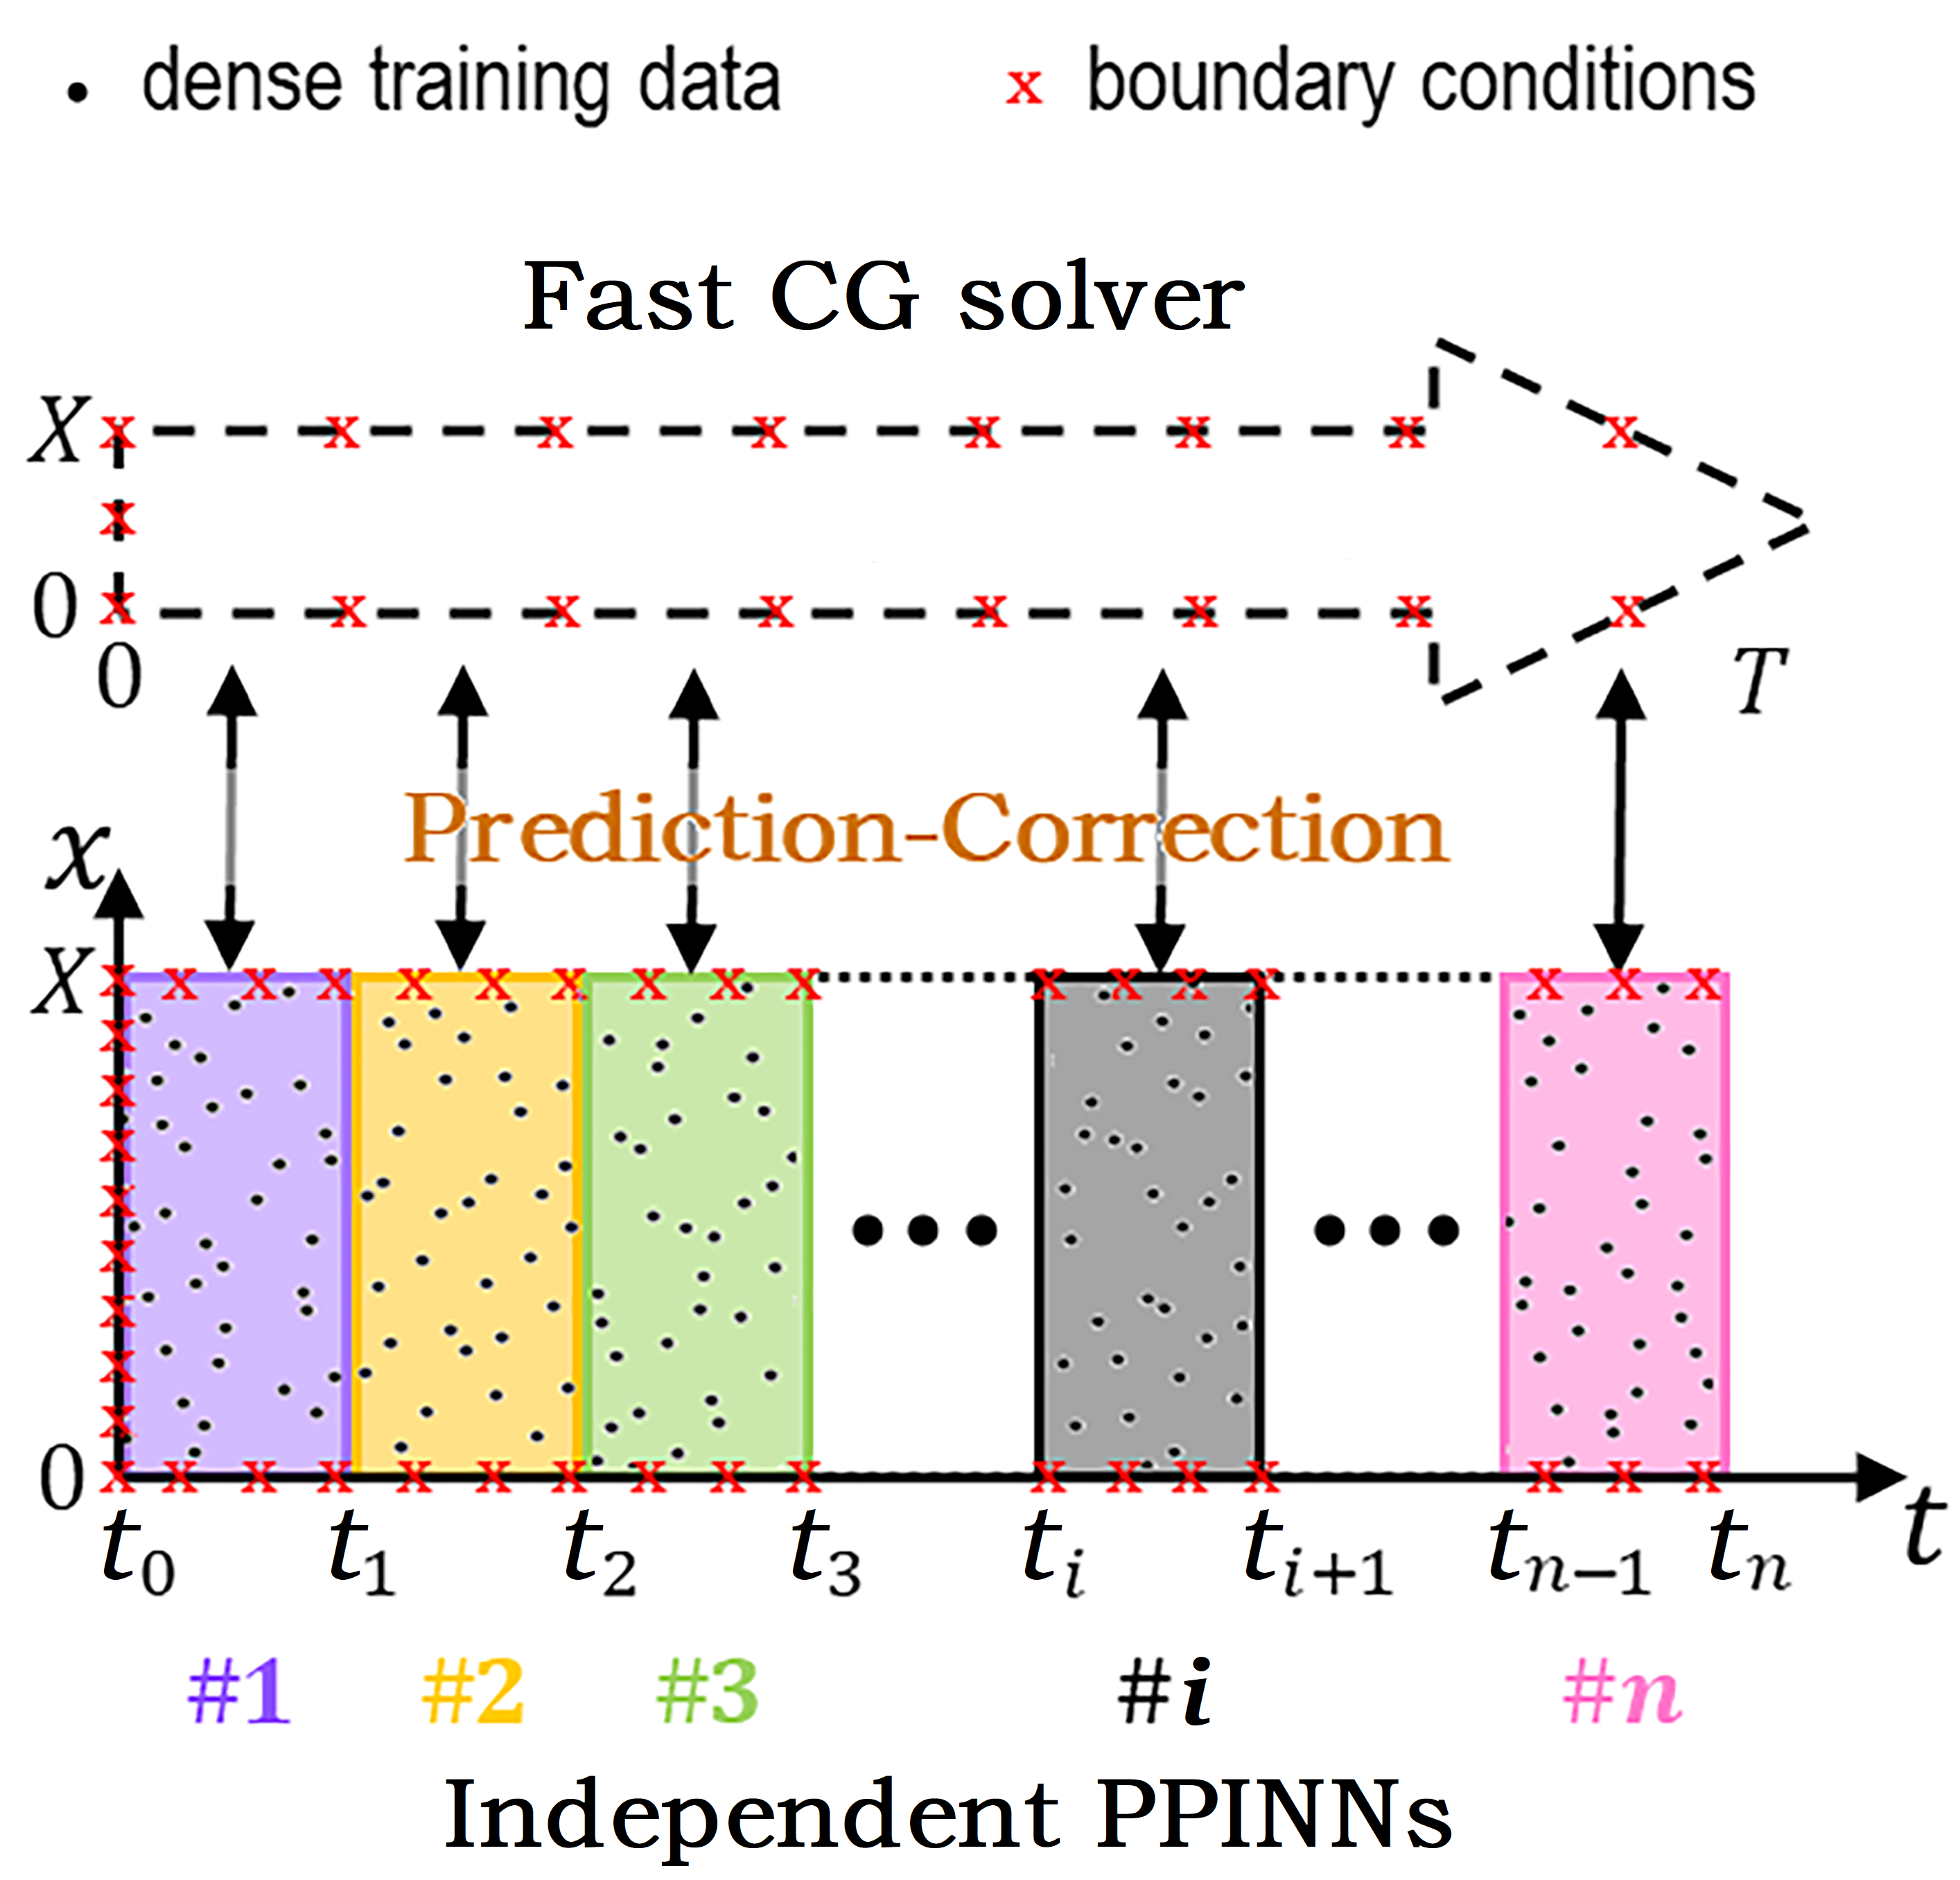
\includegraphics[scale=0.15]{figures/Figure2a.png}
  \caption{Schematic of the PPINN, where a long-time problem (PINN with full-sized data) is split into many independent short-time problems (PINN with small-sized data) guided by a fast coarse-grained (CG) solver.\cite{meng2020ppinn}}
\end{figure}

\begin{figure*}
    \centering
    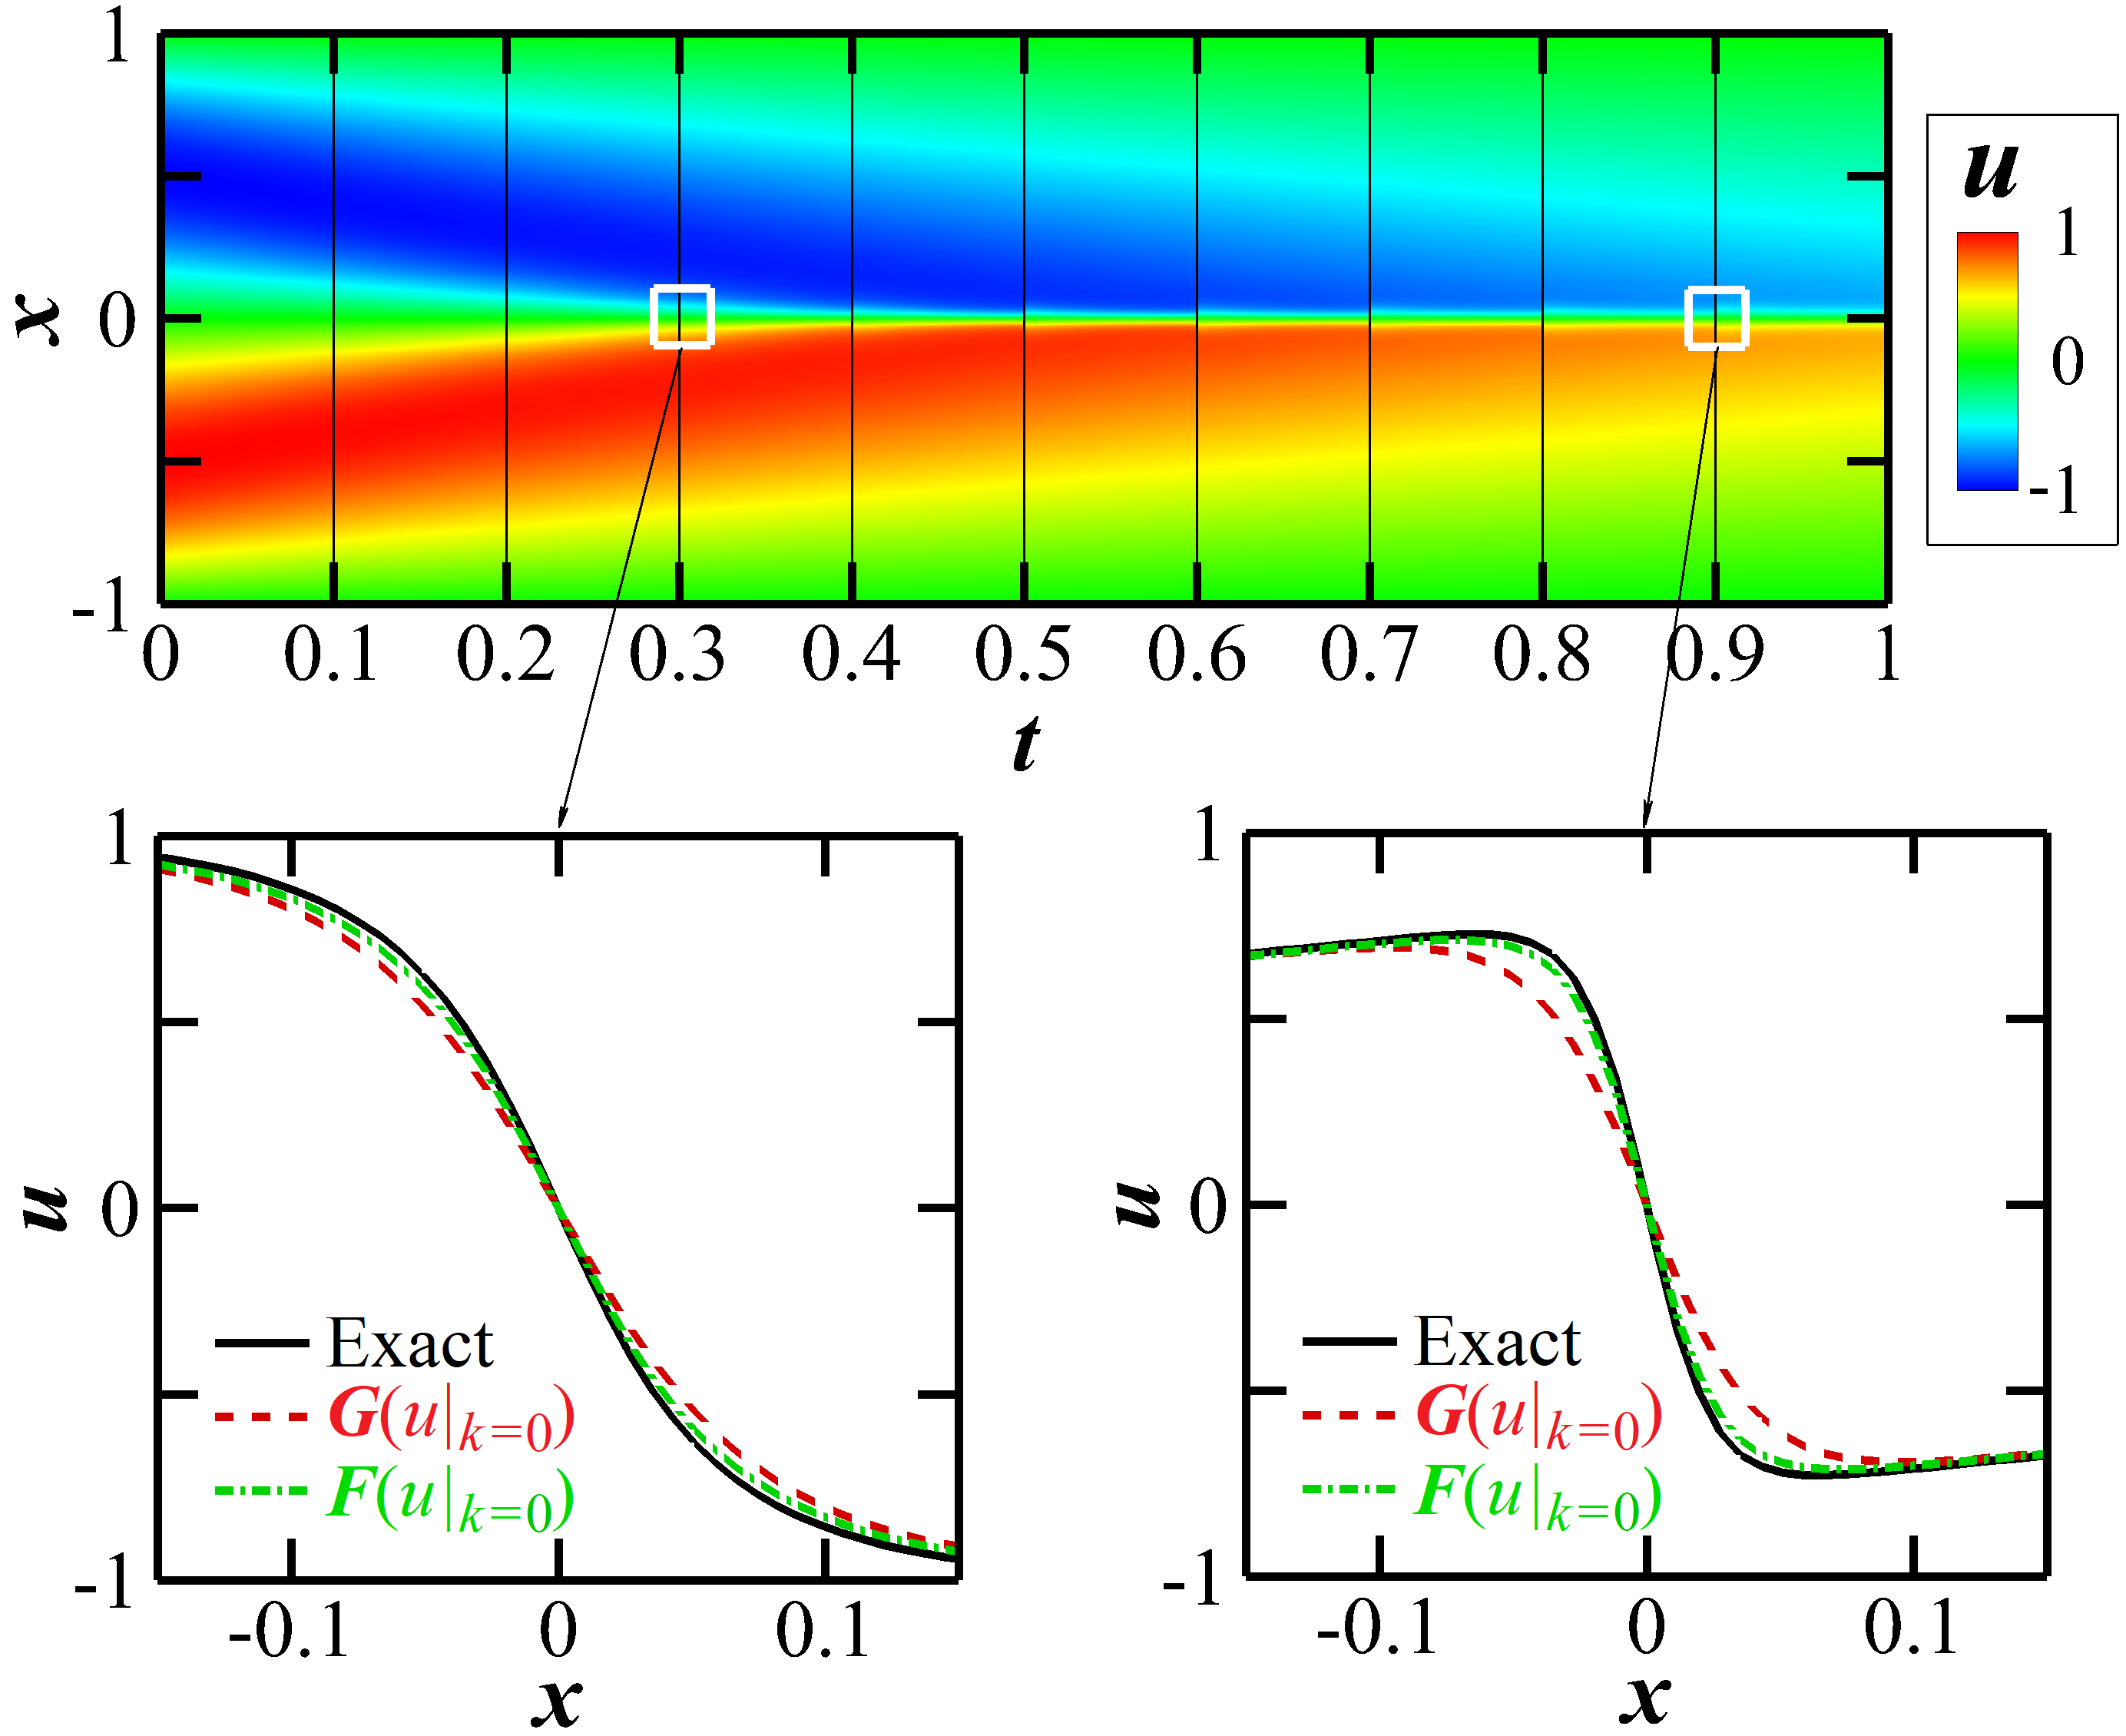
\includegraphics[scale=0.15]{figures/Figure4A.png}
    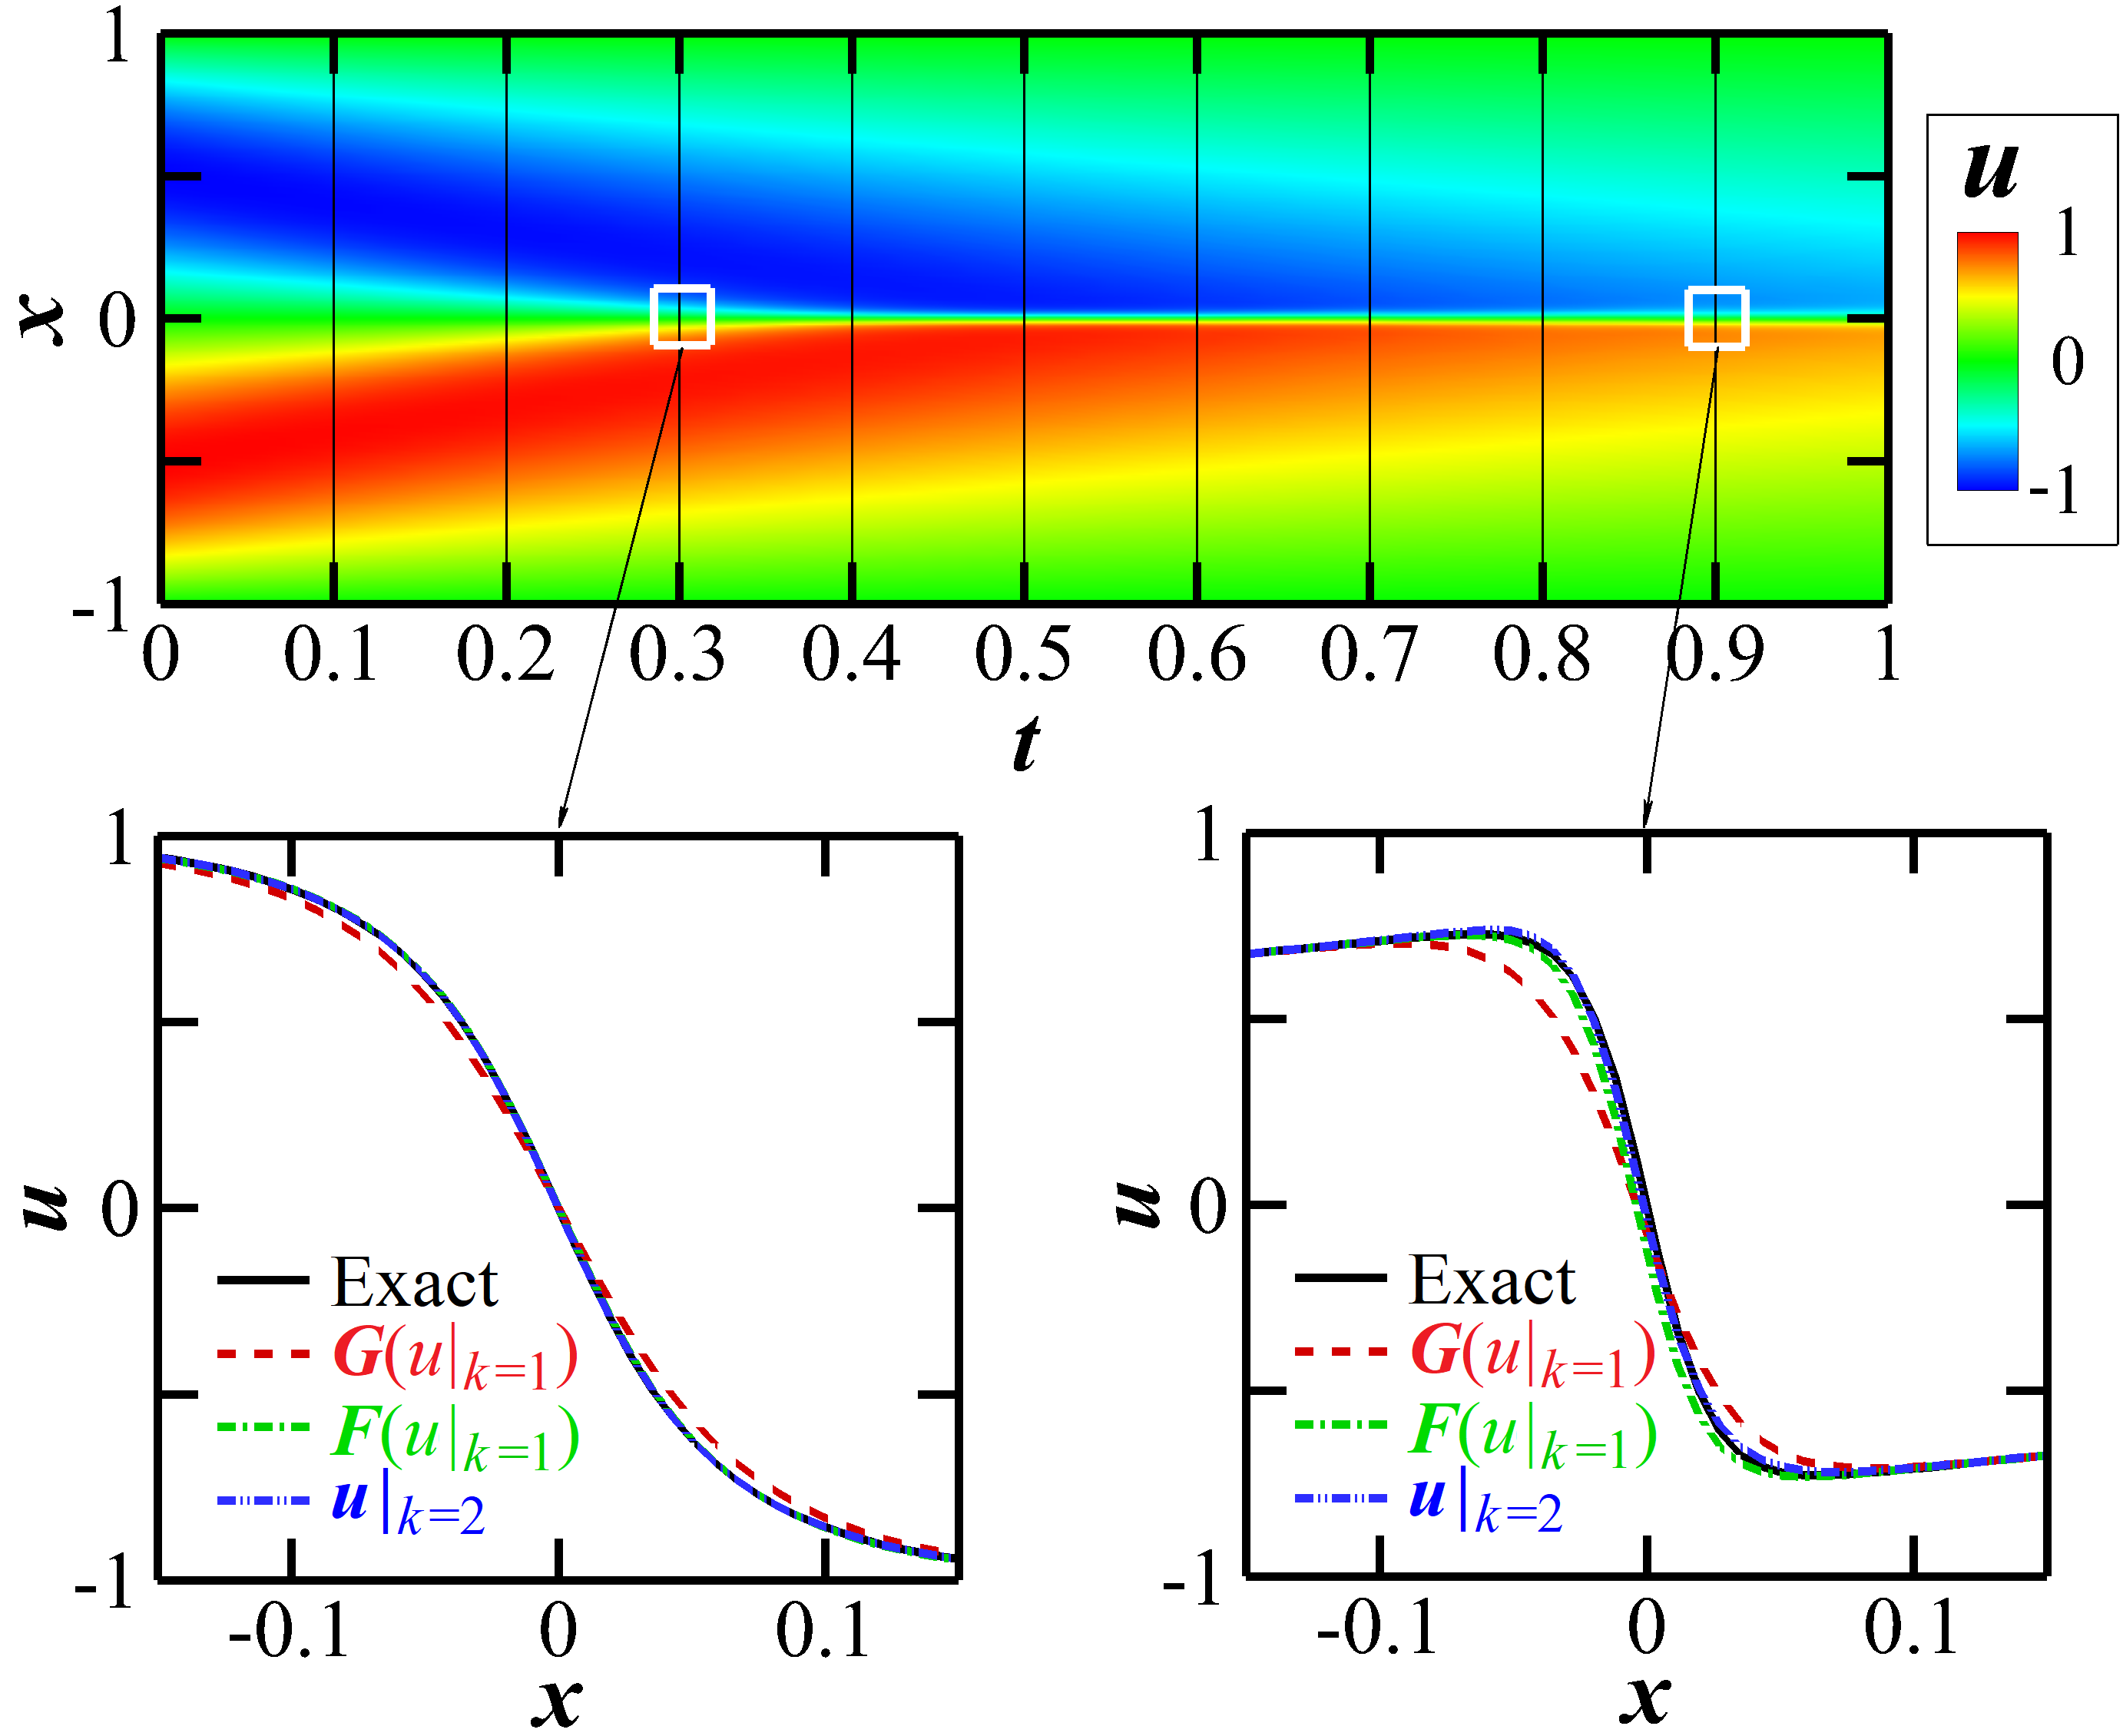
\includegraphics[scale=0.15]{figures/Figure4B.png}
     \caption{Example of using the PPINN for solving the Burgers equation.$\mathcal{G}(u(t)|_k)$ represents the rough prediction generated by the CG PINN in the $(k+1)$-th iteration, while $\mathcal{F}(u(t)|_k)$ is the solution corrected in parallel by the fine PINNs\cite{raissi2019physics}. (a) Predictions after the first iteration $(k=0)$ at $t = 0.3$ and 0.9), (b) Predictions after the second iteration ($k=1$) at $t = 0.3$ and 0.9.\cite{meng2020ppinn}}
\end{figure*}

In the following, the PPINN method is described step-by-step:
As a first step, simplify the PDE that will be solved by the CG solver. Secondly, the CG PINN is employed to solve the sPDE serially for the entire time-domain to obtain an initial solution\cite{meng2020ppinn}. Due to the fact that less residual points can be used as well as smaller neural networks to solve the sPDE rather than the original PDE, the computational cost in the CG PINN can be significantly reduced. Thirdly, decompose the time-domain into $N$ subdomains. Assume that $\mathbf{u}_i^k$ is known for $t_k \le t_i \leq t_N$ (including $k = 0$, i.e., the initial iteration), which is employed as the initial condition to run the $N$ fine PINNs in parallel\cite{meng2020ppinn}. Once the fine solutions at all $t_i$ are obtained, the discrepancy can be computed between the coarse and fine solution at $t_i$. the CG PINN is then run serially  to update the solution $\mathbf{u}$ for each interface between two adjacent subdomains, i.e., $\mathbf{u}_{i+1}^{k+1}$. Step 3 is performed iteratively until the following criterion is satisfied 

\begin{equation}
    E = \frac{\sqrt{\sum^{N-1}_{i=0} ||\mathbf{u}_{i}^{k+1} - \mathbf{u}_{i}^{k}||^2}}{\sqrt{\sum^{N-1}_{i=0} ||\mathbf{u}_{i}^{k+1}||^2}} < E_{tol},
\end{equation}
where $E_{tol}$ is a user-defined tolerance, which is set as $1\%$ in the present study.  



\subsubsection{Results}
Consider the viscous Burgers equation
\begin{equation}\label{eq:burgers}
 \frac{\partial u}{\partial t} + u\frac{\partial u}{\partial x} = \nu \frac{\partial^2 u}{\partial x^2},
\end{equation}
which is a mathematical model for the viscous flow, gas dynamics, and traffic flow, with $u$ denoting the speed of the fluid, $\nu$ the kinematic viscosity, $x$ the spatial coordinate and $t$ the time. Given an initial condition $u(x,0)=-\sin(\pi x)$ in a domain $x\in[-1,1]$, and the boundary condition $u(\pm 1, t) = 0$ for $t\in [0,1]$, the PDE to be solved is Eq.~\eqref{eq:burgers} with a viscosity of $\nu = 0.03/\pi$. 



In the PPINN, the temporal domain $t \in [0, 1]$ is decomposed into 10 uniform subdomains\cite{meng2020ppinn}. Each subdomain has a time length $\Delta t = 0.1$. The simplified PDE for the CG PINN is also a Burgers equation, which uses the same initial and boundary conditions but with a larger viscosity $\nu_c = 0.05/\pi$. It is well known that the Burgers equation with a small viscosity will develop steep gradient in its solution as time evolves.  The increased viscosity will lead to a smoother solution, which can be captured using much less computational cost\cite{meng2020ppinn}. Here, the same NN is used for the CG and fine PINNs for each subdomain, i.e., 3 hidden layers with 20 neurons per layer.


When calculating the $MSE_R$ for each subdomain's CG PINN, 300 randomly selected residual points are utilized, whereas 1,500 randomly sampled residual points are used for each subdomain's fine PINN to calculate the $MSE_{IC}$ for each subdomain, 100 equally distributed points are utilized, and 10 randomly selected points are used to calculate the $MSE_{BC}$ for both the CG and fine PINNs. 

For this particular case, it takes only 2 iterations to meet the convergence criterion, i.e., $E_{tol} = 1 $. The distributions of the $u$ at each iteration are plotted in Fig 12. As shown in Fig 12, the solution from the fine PINNs ($\mathcal{F}(u|_{k=0})$) is different from the exact one, but the discrepancy is observed to be small\cite{meng2020ppinn}.The CG PINN solution is also smoother than the fine PINN solution, especially for large-time solutions. En outre, due to incorrect beginning conditions for each domain in the first iteration, velocity at interfaces of adjoining subdivisions is not continuous. This validates the PPINN's effectiveness\cite{meng2020ppinn}. There is also a considerable reduction in the discontinuity between neighboring subdomains. Finally, it's noteworthy to note that the number of training steps for each subdomain at the first iteration ranges from tens of thousands to a few hundred for the second\cite{meng2020ppinn}.






\section{Conclusion}
This review discussed the different approaches to the idea of incorporating physics knowledge into neural network. Four architectures were discussed along with Vanilla PINNs.It was found that the main aim of more complex architecture provide better results compared to Vanilla PINNs without increasing computational costs. Architecture such as physics informed GANs and Bayesian PINNs focus on uncertainty quantification in PINNs whereas XPINNs and PPINNs focus on making the neural network fast converging and efficient.
 Since physics informed machine learning is a relatively new field of study, the research is under progress with lots of new promising results which is an assurance that the best is yet to come.

% use section* for acknowledgment
\ifCLASSOPTIONcompsoc
  % The Computer Society usually uses the plural form
  \subsection*{Acknowledgments}
\else
  % regular IEEE prefers the singular form
  \subsection*{Acknowledgment}
\fi


The author would like to thank Prof. Marlon Nuske and Prof.  Mateus Dias Ribeiro for their guidance throughout the process of writing this report and DFKI for providing this opportunity under AI Seminar SS-2021.


% trigger a \newpage just before the given reference
% number - used to balance the columns on the last page
% adjust value as needed - may need to be readjusted if
% the document is modified later
%\IEEEtriggeratref{8}
% The "triggered" command can be changed if desired:
%\IEEEtriggercmd{\enlargethispage{-5in}}

% references section

\bibliographystyle{IEEEtran}

\bibliography{pinn} 

% that's all folks
\end{document}


